\documentclass[handout]{beamer}


%%%%%%%%%%%%%%%%%%%%%%%%%%%%%%%%%%%%%%%%%%%%%%%%%%%%%%%%%%%%%%%%%%%%%%%%%%%%%%%%%%%%%%%%%%%%%%%%
%
% To do
%Href
%3- Code to be inserted from files
%4- Code to be enhanced.
%5- List of figures to be added
%6- List of code to be added
%introduction to be edited
%
%%%%%%%%%%%%%%%%%%%%%%%%%%%%%%%%%%%%%%%%%%%%%%%%%%%%%%%%%%%%%%%%%%%%%%%%%%%%%%%%%%%%%%%%%%%%%%%%



%%%%%%%%%%%%%%%%%%%%%%%%%%%%%%%%%%%%%%%%%%%%%%%%%%%%%%%%%%%%%%%%%%%%%%%%%%%%%%%%%%%%%%%%%%%%%%%%
%
% Packages Definition
%
%%%%%%%%%%%%%%%%%%%%%%%%%%%%%%%%%%%%%%%%%%%%%%%%%%%%%%%%%%%%%%%%%%%%%%%%%%%%%%%%%%%%%%%%%%%%%%%%
\usepackage{listings}
\usepackage{hyperref}
\usepackage{pgf,pgfpages}
\usepackage{graphicx}
\usepackage{units}
\usepackage[utf8]{inputenc}
\usepackage{pstricks}
\usepackage{multicol}
\usepackage{caption} % improved spacing between figure and caption

\DeclareCaptionLabelSeparator{horse}{:\quad} % change according to your needs
\captionsetup{
	labelsep = horse,
	figureposition = bottom
} 


%%%%%%%%%%%%%%%%%%%%%%%%%%%%%%%%%%%%%%%%%%%%%%%%%%%%%%%%%%%%%%%%%%%%%%%%%%%%%%%%%%%%%%%%%%%%%%%%
%
% To Add hyperlink setup
%
%%%%%%%%%%%%%%%%%%%%%%%%%%%%%%%%%%%%%%%%%%%%%%%%%%%%%%%%%%%%%%%%%%%%%%%%%%%%%%%%%%%%%%%%%%%%%%%%

\hypersetup{colorlinks=false,
	linkbordercolor=red,
	linkcolor=green,
	pdfborderstyle={/S/B/W 1}
}


%%%%%%%%%%%%%%%%%%%%%%%%%%%%%%%%%%%%%%%%%%%%%%%%%%%%%%%%%%%%%%%%%%%%%%%%%%%%%%%%%%%%%%%%%%%%%%%%
% 
% To add sections numbers to table of content
%
%%%%%%%%%%%%%%%%%%%%%%%%%%%%%%%%%%%%%%%%%%%%%%%%%%%%%%%%%%%%%%%%%%%%%%%%%%%%%%%%%%%%%%%%%%%%%%%%


\setbeamertemplate{section in toc}[sections numbered]
\setbeamercolor{section in toc}{fg=blue}

\setbeamertemplate{subsection in toc}[subsections numbered]
\setbeamercolor{subsection in toc}{fg=blue}

\defbeamertemplate{subsubsection in toc}{subsubsections numbered}
{\leavevmode\leftskip=3em%
	\rlap{\hskip-3em\inserttocsectionnumber.\inserttocsubsectionnumber.\inserttocsubsubsectionnumber}%
	\inserttocsubsubsection\par}

\setbeamertemplate{subsubsection in toc}[subsubsections numbered]
\setbeamercolor{subsubsection in toc}{fg=blue}




%%%%%%%%%%%%%%%%%%%%%%%%%%%%%%%%%%%%%%%%%%%%%%%%%%%%%%%%%%%%%%%%%%%%%%%%%%%%%%%%%%%%%%%%%%%%%%%%
%
% To add the list of figures at the end of slides
%
%%%%%%%%%%%%%%%%%%%%%%%%%%%%%%%%%%%%%%%%%%%%%%%%%%%%%%%%%%%%%%%%%%%%%%%%%%%%%%%%%%%%%%%%%%%%%%%%

%\makeatletter
%
%\AtEndDocument{%
%	\clearpage
%	\beamer@tempcount=\c@page\advance\beamer@tempcount by -1%
%	\if@filesw
%	\immediate\write\@auxout{\string\@writefile{lof}%
%		{\noexpand\headcommand{\noexpand\beamer@partpages{\the\beamer@partstartpage}{\the\beamer@tempcount}}}}%
%	\newwrite\tf@lof
%	\immediate\openout\tf@lof\jobname.lof\relax
%	\immediate\write\@auxout{\string\@writefile{lot}%
%		{\noexpand\headcommand{\noexpand\beamer@partpages{\the\beamer@partstartpage}{\the\beamer@tempcount}}}}%
%	\newwrite\tf@lot
%	\immediate\openout\tf@lot\jobname.lof\relax
%	\fi
%}
%
%\long\def\beamer@makecaption#1#2{%
%	\def\insertcaptionname{\csname#1name\endcsname}%
%	\def\insertcaptionnumber{\csname the#1\endcsname}%
%	\def\insertcaption{#2}%
%	\def\@tempa{#1}
%	\def\@tempb{figure}
%	\ifx\@tempa\@tempb
%	\addtocontents{lof}{\protect\listoffigureformat{\insertcaptionnumber}{\insertcaption}}{}{}%
%	\else
%	\addtocontents{lot}{\protect\listoffigureformat{\insertcaptionnumber}{\insertcaption}}{}{}%
%	\fi%
%	\nobreak\vskip\abovecaptionskip\nobreak
%	\sbox\@tempboxa{\usebeamertemplate**{caption}}%
%	\ifdim \wd\@tempboxa >\hsize
%	\usebeamertemplate**{caption}\par
%	\else
%	\global \@minipagefalse
%	\hb@xt@\hsize{\hfil\box\@tempboxa\hfil}%
%	\fi
%	\nobreak\vskip\belowcaptionskip\nobreak}
%
%\def\listoffigureformat#1#2{#1:~#2\par}
%\def\listoffigures{%
%	\frame{\frametitle{List of Figures}
%		\@starttoc{lof}%
%	}
%}
%\makeatother
%
%

%%%%%%%%%%%%%%%%%%%%%%%%%%%%%%%%%%%%%%%%%%%%%%%%%%%%%%%%%%%%%%%%%%%%%%%%%%%%%%%%%%%%%%%%%%%%%%%%
%
% To define Code Syntax Matlab,Scala
%
%%%%%%%%%%%%%%%%%%%%%%%%%%%%%%%%%%%%%%%%%%%%%%%%%%%%%%%%%%%%%%%%%%%%%%%%%%%%%%%%%%%%%%%%%%%%%%%%


%%%%%%%%%%%%%%%%%%%%%%%%%%%%%%%%%%%%%%%%%%%%%%%%%%%%%%%%%%%%%%%%%%%%%%%%%%%%%%%%%%%%%%%%%%%%%%%%
%
% Matlab
%
%%%%%%%%%%%%%%%%%%%%%%%%%%%%%%%%%%%%%%%%%%%%%%%%%%%%%%%%%%%%%%%%%%%%%%%%%%%%%%%%%%%%%%%%%%%%%%%%


%\lstloadlanguages{Matlab}
%\lstset{language=Matlab, xleftmargin=0pt, numberstyle=\tiny, numbersep=0pt, breaklines=true, breakindent=20pt, commentstyle=\scriptsize, frame=single, frameround=tttt}
%\renewcommand{\lstlistingname}{
%\textbf{\underline{Matlab Code}}}

%%%%%%%%%%%%%%%%%%%%%%%%%%%%%%%%%%%%%%%%%%%%%%%%%%%%%%%%%%%%%%%%%%%%%%%%%%%%%%%%%%%%%%%%%%%%%%%%
%
% Scala
%
%%%%%%%%%%%%%%%%%%%%%%%%%%%%%%%%%%%%%%%%%%%%%%%%%%%%%%%%%%%%%%%%%%%%%%%%%%%%%%%%%%%%%%%%%%%%%%%%

\lstdefinestyle{myScalastyle}{
  frame=tb,
  language=scala,
  aboveskip=3mm,
  belowskip=3mm,
  showstringspaces=false,
  columns=flexible,
  numbers=left,                   % where to put the line-numbers
  numberstyle=\tiny\color{gray},  % the style that is used for the line-numbers
  stepnumber=1,                   % the step between two line-numbers. If it's 1, each line will be numbered
  numbersep=5pt,                  % how far the line-numbers are from the code
  backgroundcolor=\color{white},  % choose the background color. You must add 
  keywordstyle=\color{blue},
  commentstyle=\color{mygreen},
%  stringstyle=\color{mauve},
  stringstyle=\color{myorange},
  frame=single,
  breaklines=true,
  breakatwhitespace=true,
  breakindent=20pt,
  tabsize=3,
  frameround=tttt,
  escapeinside={\%*}{*)},        % to add a comment within your code
  emph={count,take,textFile,filter,first,collect,mkString}, % Scala functions
  emphstyle={\color{mauve}},
  morekeywords ={val,sc},        % to add more keywords to the set  
}
\renewcommand{\lstlistingname}{\textbf{\underline{Scala Code}}}

%%%%%%%%%%%%%%%%%%%%%%%%%%%%%%%%%%%%%%%%%%%%%%%%%%%%%%%%%%%%%%%%%%%%%%%%%%%%%%%%%%%%%%%%%%%%%%%%



% % % % % % % % % % % % % % % % % % % % % % % % % % % % % % % % % % % % % % % % % % % % % % % % %

\mode<presentation>
{
  \usetheme{ift}
%    \usetheme{Goettingen}
  
%  \usetheme{Luebeck}
  \setbeamercovered{transparent}
  \setbeamertemplate{items}[square]
}


\usefonttheme[onlymath]{serif}
\setbeamerfont{frametitle}{size=\LARGE,series=\bfseries}

%%%%%%%%%%%%%%%%%%%%%%%%%%%%%%%%%%%%%%%%%%%%%%%%%%%%%%%%%%%%%%%%%%%%%%%%%%%%%%%%%%%%%%%%%%%%%%%%
% 
% To define sime custom colors
%
%%%%%%%%%%%%%%%%%%%%%%%%%%%%%%%%%%%%%%%%%%%%%%%%%%%%%%%%%%%%%%%%%%%%%%%%%%%%%%%%%%%%%%%%%%%%%%%%


%\definecolor{uibred}{RGB}{170, 0, 0}
%\definecolor{uibblue}{RGB}{0, 84, 115}
%\definecolor{uibgreen}{RGB}{119, 175, 0}
%\definecolor{uibgreen}{RGB}{50, 105, 0}
\definecolor{uiborange}{RGB}{217, 89, 0}
\definecolor{MyGray}{rgb}{.9, .9, .9}
\definecolor{myorange}{rgb}{1.0,0.4,0}
\definecolor{mygreen}{rgb}{0,0.8,0.6}
\definecolor{dkgreen}{rgb}{0,0.6,0}
\definecolor{gray}{rgb}{0.5,0.5,0.5}
\definecolor{mauve}{rgb}{0.58,0,0.82}

%%%%%%%%%%%%%%%%%%%%%%%%%%%%%%%%%%%%%%%%%%%%%%%%%%%%%%%%%%%%%%%%%%%%%%%%%%%%%%%%%%%%%%%%%%%%%%%%



\beamertemplatenavigationsymbolsempty

%====================================================
%-------------Macro definitions go here--------------
%====================================================

%
% Differentials
%
\newcommand{\tdiff}[2]{\ensuremath{\frac{\mathrm{d}#2}}{\mathrm{d}{#1}}}
\newcommand{\tdifforder}[3]{\ensuremath{\frac{\mathrm{d}^{#2}#3}{\mathrm{d}{#1}^{#2}}}}
\newcommand{\pdiff}[2]{\ensuremath{\frac{\partial#2 }{\partial#1}}}
\newcommand{\pdifforder}[3]{\ensuremath{\frac{\partial^{#2}#3}{\partial{#1}^{#2}}}}

% bracket
\newcommand{\bra}[1]{\ensuremath{\left<#1\right|}}
\newcommand{\ket}[1]{\ensuremath{\left|#1\right>}}
\newcommand{\bracket}[2]{\ensuremath{ \left\langle #1 | #2 \right\rangle}}
\newcommand{\matelem}[3]{\ensuremath{ \left\langle #1 | #2 | #3 \right\rangle}}
\newcommand{\matr}[1]{\ensuremath{\mathbf{#1}}}
\newcommand{\vect}[1]{\ensuremath{\mathbf{#1}}}
\newcommand{\expectationvalue}[1]{\ensuremath{\left\langle #1 \right\rangle}}

\renewcommand{\imath}{\ensuremath{\mathrm{i}}}

%
% Linear algebra
%
\renewcommand{\vec}[1]{\ensuremath{\mathbf{#1}}}
\newcommand{\mat}[1]{\ensuremath{\mathbf{#1}}}
\newcommand{\tildemat}[1]{\ensuremath{\widetilde{\mat{#1}}}}

% Numerical analysis
\newcommand{\bigo}{\ensuremath{\mathcal{O}}}
\renewcommand{\Re}{\ensuremath{\mathrm{Re}}}
\renewcommand{\Im}{\ensuremath{\mathrm{Im}}}
\newcommand{\mathcol}[2]{{\color{#1}#2}}
%\newcommand{\red}[1]{\mathcol{uibred}{#1}}
%\newcommand{\blue}[1]{\mathcol{uibblue}{#1}}
%\newcommand{\green}[1]{\mathcol{uibgreen}{#1}}
\newcommand{\orange}[1]{\mathcol{uiborange}{#1}}
%
% Misc macros
%
\newcommand{\eref}[1]{~(\ref{#1})}
\renewcommand{\equiv}[0]{\ensuremath{:=}}
\newcommand{\etal}{\textit{et al. }}
\newcommand{\paperheader}[2]{\noindent\textbf{Paper #1}: \textit{#2}\\}
\newcommand{\paperitem}[3]{\noindent\textbf{Paper #1}: \textit{#2}\vspace{1em}\\\noindent #3\vspace{2em}}
\newcommand{\tfinal}{\ensuremath{T_{\text{f}}}}
\newcommand{\papernum}[1]{\textbf{#1}}
%\newcommand{\note}[1]{\colorbox{yellow}{#1}}
\newcommand{\paperref}[1]{Paper~\textbf{#1}}

%
% Code
%
\newcommand{\inlinename}[1]{\lstinline[basicstyle=\ttfamily,language=bash]{#1}}



%\Includeonlyframes{current}

\newcommand{\ShowGraphics}

%%%%%%%%%%%%%%%%%%%%%%%%%%%%%%%%%%%%%%%%%%%%%%%%%%%%%%%%%%%%%%%%%%%%%%%%%%%%%%%%%%%%%%%%%%%%%%%%
% 
% To Pass graphics paths
%
%%%%%%%%%%%%%%%%%%%%%%%%%%%%%%%%%%%%%%%%%%%%%%%%%%%%%%%%%%%%%%%%%%%%%%%%%%%%%%%%%%%%%%%%%%%%%%%%

\graphicspath{{./Ch02SparkDataProcessing/}{./Graphics/}}


%%%%%%%%%%%%%%%%%%%%%%%%%%%%%%%%%%%%%%%%%%%%%%%%%%%%%%%%%%%%%%%%%%%%%%%


\defbeamertemplate{enumerate item}{mycircle}
{
  %\usebeamerfont*{item projected}%
  %\usebeamercolor[bg]{item projected}%
  \begin{pgfpicture}{0ex}{0ex}{1.5ex}{0ex}
	%\pgfcircle[fill]{\pgfpoint{0pt}{.75ex}}{1.25ex}
    \pgfbox[center,base]{\color{uibblue}\insertenumlabel.}
  \end{pgfpicture}%
}


%%%%%%%%%%%%%%%%%%%%%%%%%%%%%%%%%%%%%%%%%%%%%%%%%%%%%%%%%%%%%%%%%%%%%%%%%%%%%%%%%%%%%%%%%%%%%%%%
% 
% Bio
%
%%%%%%%%%%%%%%%%%%%%%%%%%%%%%%%%%%%%%%%%%%%%%%%%%%%%%%%%%%%%%%%%%%%%%%%%%%%%%%%%%%%%%%%%%%%%%%%%


\title{Big Data Processing :\\ Using Spark}
\author{Mostafa Alaa Mohamed\\ Senior Big Data Engineer \\ Email: \href{mailto: mustafaalaa.mohamed@gmail.com}{mustafaalaa.mohamed@gmail.com} \\ Linkedin: \href{https://www.linkedin.com/in/mostafa-alaa-5120615b/}{Mostafa Alaa} }
\institute{
Big Data \& Analytics Department, Etisalat UAE
}
\date{\gray \today}

%%%%%%%%%%%%%%%%%%%%%%%%%%%%%%%%%%%%%%%%%%%%%%%%%%%%%%%%%%%%%%%%%%%%%%%%%%%%%%%%%%%%%%%%%%%%%%%%
% 
% begin document
%
%%%%%%%%%%%%%%%%%%%%%%%%%%%%%%%%%%%%%%%%%%%%%%%%%%%%%%%%%%%%%%%%%%%%%%%%%%%%%%%%%%%%%%%%%%%%%%%%



\begin{document}

\begin{frame}
  \titlepage
  \vspace{5cm}
\end{frame}

\begin{frame}
	  \frametitle{Table of Content:}
	\tableofcontents
\end{frame}
%\begin{frame}
%	\frametitle{List of figures:}
%%	\listoffigures
%\lstlistoflistings
%
%\end{frame}



%
% Set the background for the rest of the slides.
% Insert info line at the end
%
\setbeamertemplate{background}
{
\includegraphics[width=\paperwidth,height=\paperheight]{nabil_slide_helwan_bg}}
\setbeamertemplate{footline}[ifttheme]

\setbeamertemplate{caption}[numbered]


%%%%%%%%%%%%%%%%%%%%%%%%%%%%%%%%%%%%%%%%%%%%%%%%%%%%%%%%%%%%%%%%%%%%%%%%%%%%%%%%%%%%%%%%%%%%%%%%%%
%
% Insert Front Page
%
%%%%%%%%%%%%%%%%%%%%%%%%%%%%%%%%%%%%%%%%%%%%%%%%%%%%%%%%%%%%%%%%%%%%%%%%%%%%%%%%%%%%%%%%%%%%%%%%%%

%\input{FrontMatter/FrontMatter.tex}


%%%%%%%%%%%%%%%%%%%%%%%%%%%%%%%%%%%%%%%%%%%%%%%%%%%%%%%%%%%%%%%%%%%%%%%%%%%%%%%%%%%%%%%%%%%%%%%%%%
%
%\section{Introduction}

%%%%%%%%%%%%%%%%%%%%%%%%%%%%%%%%%%%%%%%%%%%%%%%%%%%%%%%%%%%%%%%%%%%%%%%%%%%

\begin{frame}
  \frametitle{Introduction To Spark}
%%TCIMACRO{To adapt the Image size}%


\includegraphics[width=\textwidth,height=7cm]{Graphics/Dist.jpg}

\end{frame}

%%%%%%%%%%%%%%%%%%%%%%%%%%%%%%%%%%%%%%%%%%%%%%%%%%%%%%%%%%%%%%%%%%%%%%%%%%%
\begin{frame}
  \frametitle{Introduction To Spark}
	\begin{itemize}[<+->]
		\item Any Big Data solution working based distributed systems.
		\item What is distributed systems in brief?
			\begin{itemize}
					\item Components interact with each other in order to achieve a common goal.
					\item Problem definition is to run a process and distribute it into Multi node.
					\item Every system has its own way to manage the cluster (distributed system). Managing the cluster including 
						\begin{itemize}
							\item How the data will be processed.
							\item How the data will be shuffling (transferring) between the nodes .
							\item Keep track of the current processing tasks.
							\item Handle the logs and long running tasks.
						\end{itemize}
			\end{itemize}
	\end{itemize}
\end{frame}

%%%%%%%%%%%%%%%%%%%%%%%%%%%%%%%%%%%%%%%%%%%%%%%%%%%%%%%%%%%%%%%%%%%%%%%%%%%

\section{What Is Apache Spark?}
\begin{frame}
  \frametitle{Introduction To Spark}
	\begin{itemize}[<+->]
		\item Apache Spark is Fast and general cluster computing engine that extends Google’s MapReduce model
		\item Write programs in terms of parallel transformations on distributed datasets.
		\item The power of supporting research in the Labs gained Spark. How? \\ \textit{Apache Spark is an open source big data processing framework built around speed, ease of use, and sophisticated analytics. It was originally developed in 2009 in UC Berkeley’s \textbf{AMPLab}, and open sourced in 2010 as an Apache project.}

	\end{itemize}%

\end{frame}

%%%%%%%%%%%%%%%%%%%%%%%%%%%%%%%%%%%%%%%%%%%%%%%%%%%%%%%%%%%%%%%%%%%%%%%%%%%%
\begin{frame}
  \frametitle{Introduction To Spark}
		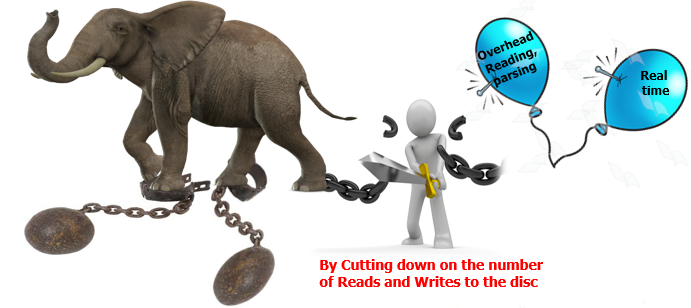
\includegraphics[width=\textwidth,height=7cm]{Graphics/Sparkvsmapreduce.png}
\end{frame}


%%%%%%%%%%%%%%%%%%%%%%%%%%%%%%%%%%%%%%%%%%%%%%%%%%%%%%%%%%%%%%%%%%%%%%%%%%%%
\begin{frame}
  \frametitle{Introduction To Spark}
	\begin{itemize}[<+->]
		\item Improves efficiency through: In-memory data sharing, General computation graphs(100x faster).
		\item Improves usability through: Rich APIs in Java, Scala, Python, Interactive shell(2-5x less code)
	\end{itemize}
\end{frame}

%%%%%%%%%%%%%%%%%%%%%%%%%%%%%%%%%%%%%%%%%%%%%%%%%%%%%%%%%%%%%%%%%%%%%%%%%%%%

\section{Example Spark vs Mapreduce on Hadoop}
\begin{frame}[fragile]
	\frametitle{Example Mapreduce on Hadoop}
%	
\includegraphics[width=3cm]{Graphics/Hadoop.PNG}

\begin{lstlisting}[style=myScalastyle, caption=Java Mapreduce Average Example]
private IntWritable one = new IntWritable(1);
private IntWritable output = new IntWritable()
proctected void map(LongWritable key,Text value, Context context) 
{String[] fields = value.split("\t");
output.set(Integer.parseInt(fields[1]));
context.write(one, output);}
IntWritable one = new IntWritable(1);
DoubleWritable average = new DoubleWritable();
protected void reduce(IntWritable key,Iterable<IntWritable> values,Context context) {
int sum = 0 ; int count = 0;
for(IntWritable value : values) {
sum += value.get(); count++;}
average.set(sum / (double) count);
context.Write(key, average);}
\end{lstlisting}

%\lstinputlisting[language=java]{"AVGExample.java"}
\end{frame}

%%%%%%%%%%%%%%%%%%%%%%%%%%%%%%%%%%%%%%%%%%%%%%%%%%%%%%%%%%%%%%%%%%%%%%%%%%%%
\begin{frame}[fragile]
	\frametitle{Example Spark on Hadoop}
	
\includegraphics[width=3cm]{Graphics/spark.jpg}
	
%	\begin{minted}{python}
	
\begin{lstlisting}[language=Python, caption=Python Spark Average Example]
	data = sc.textFile(...).split("\t")
	data.map(lambda x: (x[0], [x.[1], 1])) \
	.reduceByKey(lambda x, y: [x[0] + y[0], x[1] + y[1]]) \
	.map(lambda x: [x[0], x[1][0] / x[1][1]]) \
	.collect()	
\end{lstlisting}
%\end{minted}

\end{frame}

%%%%%%%%%%%%%%%%%%%%%%%%%%%%%%%%%%%%%%%%%%%%%%%%%%%%%%%%%%%%%%%%%%%%%%%%%%%%
\section{Downloading Spark and Getting Started.} 
\subsection{Installing Apache Spark and Scala}
\begin{frame}
	\frametitle{Installing Apache Spark and Scala}
	please refer to this article and videos below
	\begin{itemize}[<+->]
	\item \href{https://github.com/MostafaAlaa2016/Spark\_Installation}{\color{blue}Github Document}.
	\item \href{https://www.youtube.com/watch?v=WlE7RNdtfwE}{\color{blue}Youtube Video}.
	\end{itemize}
\end{frame}


%
%%%%%%%%%%%%%%%%%%%%%%%%%%%%%%%%%%%%%%%%%%%%%%%%%%%%%%%%%%%%%%%%%%%%%%%%%%%%%%%%%%%%%%%%%%%%%%%%%%

%\input{ChNabile/ChNabile.tex}

%%%%%%%%%%%%%%%%%%%%%%%%%%%%%%%%%%%%%%%%%%%%%%%%%%%%%%%%%%%%%%%%%%%%%%%%%%%%%%%%%%%%%%%%%%%%%%%%%%%%
%
\section{Programming with RDDs}
%%%%%%%%%%%%%%%%%%%%%%%%%%%%%%%%%%%%%%%%%%%%%%%%%%%%%%%%%%%%%%%%%%%%%%%%%%%
%
%
%
%%%%%%%%%%%%%%%%%%%%%%%%%%%%%%%%%%%%%%%%%%%%%%%%%%%%%%%%%%%%%%%%%%%%%%%%%%%

%\begin{frame}
%  \frametitle{Chapter overview}
%	\begin{itemize}[<+->]
%		\item How we will walk through this Chapter?
%			\begin{itemize}
%				\item what is RDD?
%				\item How to create RDD?
%				\item How to communicate between RDD and Spark API?
%				\item How Spark Distribute RDD?
%				\item What types of operation RDDs offer?
%			\end{itemize}
%	\end{itemize}
%\end{frame}

%%%%%%%%%%%%%%%%%%%%%%%%%%%%%%%%%%%%%%%%%%%%%%%%%%%%%%%%%%%%%%%%%%%%%%%%%%%
%
%
%
%%%%%%%%%%%%%%%%%%%%%%%%%%%%%%%%%%%%%%%%%%%%%%%%%%%%%%%%%%%%%%%%%%%%%%%%%%%

\subsection{RDD Basics}
\subsubsection{Spark Programming Model}
%TCIDATA%\item How to write a program to do a transformation on distributed datasets?

\begin{frame}
  \frametitle{Resilient Distributed Datasets (RDDs)}
	\begin{itemize}[<+->]
		\item \textbf{Resilient Distributed Datasets (RDDs)}
			\begin{itemize}
				\item \textbf{Resilient}: Automatically rebuilt on failure
				\item \textbf{Distributed}: Means that transformations is done over collections of \textit{immutable objects} that can be stored in memory or disk in multi-nodes across a cluster via parallel transformations (map, filter, …)
				\item \textbf{Datasets} Initial data can come from a file or be created pragmatically
			\end{itemize}
	\item RDDs are the fundamental unit of data in Spark.
	\end{itemize}
\end{frame}
%%%%%%%%%%%%%%%%%%%%%%%%%%%%%%%%%%%%%%%%%%%%%%%%%%%%%%%%%%%%%%%%%%%%%%%%%%%
%
%
%
%%%%%%%%%%%%%%%%%%%%%%%%%%%%%%%%%%%%%%%%%%%%%%%%%%%%%%%%%%%%%%%%%%%%%%%%%%%


\subsubsection{RDD Creation}

\begin{frame}
  \frametitle{How to create RDD (1/2)}
	\begin{itemize}[<+->]
		\item \textbf{How to create RDD}?
			\begin{itemize}
				\item Loading an external dataset
				\item Distributing a collection of objects (e.g., a list or set) in their driver program
				\item From data in memory
				\item From another RDD
			\end{itemize}
	\end{itemize}
\end{frame}

\begin{frame}
	\frametitle{How to create RDD (2/2)}
	\begin{itemize}[<+->]
		\item \textbf{\underline{Important Note}}: Source of some below figures from the following link:  http://datalakes.com/rdds-simplified/
		\begin{figure}
			\caption{RDD Partitions}  		  	
			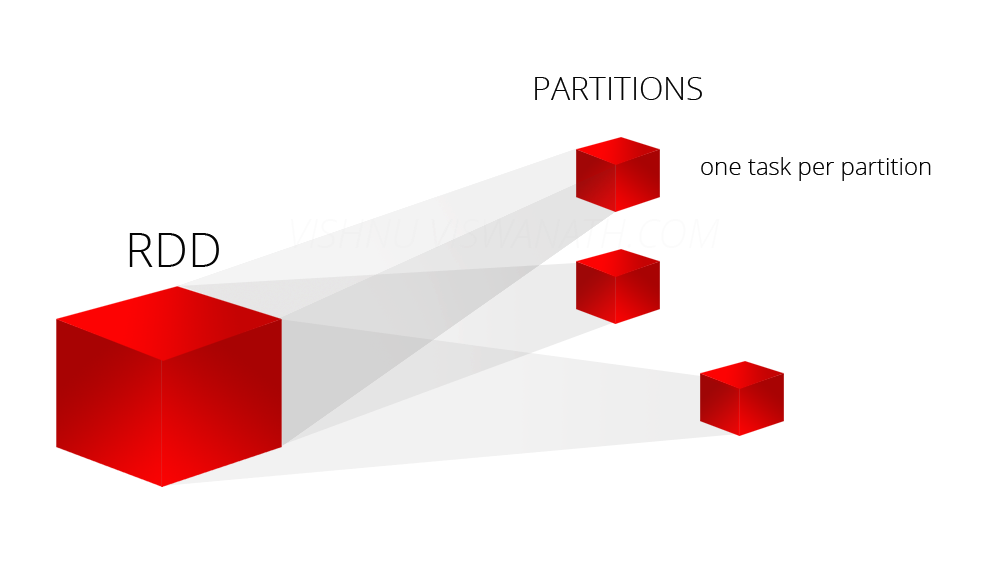
\includegraphics[width=\textwidth,height=5.5cm]{Graphics/RDD_Patitions.PNG}
		\end{figure}
		
	\end{itemize}
\end{frame}

%%%%%%%%%%%%%%%%%%%%%%%%%%%%%%%%%%%%%%%%%%%%%%%%%%%%%%%%%%%%%%%%%%%%%%%%%%%
%
%
%
%%%%%%%%%%%%%%%%%%%%%%%%%%%%%%%%%%%%%%%%%%%%%%%%%%%%%%%%%%%%%%%%%%%%%%%%%%%
\begin{frame}[fragile]
  \frametitle{Creating RDD Example:}

			\begin{lstlisting}[style=myScalastyle, caption=Creating RDD Example]
//Read READ.md File into lines 
val lines = sc.textFile("README.md")
//lines: org.apache.spark.rdd.RDD[String] = README.md MapPartitionsRDD[3] at textFile at <console>:24			
lines.take(3)
//res4: Array[String] = Array
//(# "Apache Spark", "", "Spark is a fast and general cluster computing system for Big Data. It provides")		
lines.count
//res5: Long = 99
			\end{lstlisting}

\end{frame}

%%%%%%%%%%%%%%%%%%%%%%%%%%%%%%%%%%%%%%%%%%%%%%%%%%%%%%%%%%%%%%%%%%%%%%%%%%%
%
%
%
%%%%%%%%%%%%%%%%%%%%%%%%%%%%%%%%%%%%%%%%%%%%%%%%%%%%%%%%%%%%%%%%%%%%%%%%%%%


\subsubsection{Spark Context}

\begin{frame}
  \frametitle{Spark Context:}
	\begin{itemize}[<+->]
		\item \textbf{What is Spark Context?}
			\begin{itemize}
					\item Your main entry point to spark API
					\item The way and only way to distribute the data
			\end{itemize}
	\end{itemize}
\end{frame}

%%%%%%%%%%%%%%%%%%%%%%%%%%%%%%%%%%%%%%%%%%%%%%%%%%%%%%%%%%%%%%%%%%%%%%%%%%%
%
%
%
%%%%%%%%%%%%%%%%%%%%%%%%%%%%%%%%%%%%%%%%%%%%%%%%%%%%%%%%%%%%%%%%%%%%%%%%%%%


\subsubsection{Spark Driver}

\begin{frame}
  \frametitle{Spark Driver(1/2):}
	\begin{itemize}[<+->]
		\item \textbf{What is Spark Driver?}
			\begin{itemize}
				\item It is the program that declares the operations(transformations and actions) on RDDs of data and submits to the master
				\item It is the program that creates the SparkContext, connecting to a given Spark Master "we can named as session "
				\item It prepares the context and declares the operations on the data using RDD transformations and actions
				\item It submits the serialized RDD graph to the master. 
				\item The master creates tasks out of it and submits them to the workers for execution. It coordinates the different job stages
				\item The workers is where the tasks are actually executed. They should have the resources and network connectivity required to execute the operations requested on the RDDs
			\end{itemize}
	\end{itemize}
\end{frame}


%%%%%%%%%%%%%%%%%%%%%%%%%%%%%%%%%%%%%%%%%%%%%%%%%%%%%%%%%%%%%%%%%%%%%%%%%%%
%
%
%
%%%%%%%%%%%%%%%%%%%%%%%%%%%%%%%%%%%%%%%%%%%%%%%%%%%%%%%%%%%%%%%%%%%%%%%%%%%


\begin{frame}
  \frametitle{Spark Driver(2/2):}
  \begin{figure}
  	  \caption{Spark Internal Interaction}  	
	   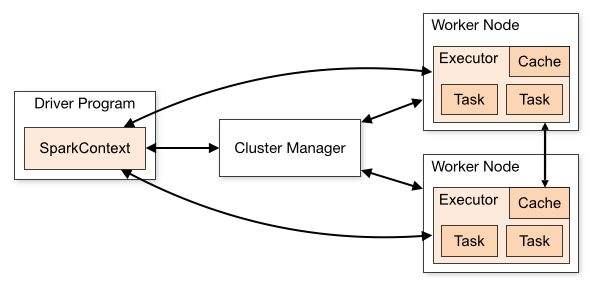
\includegraphics[width=\textwidth]{Graphics/Spark_Driver_Issue.PNG}
\end{figure}

\end{frame}


%%%%%%%%%%%%%%%%%%%%%%%%%%%%%%%%%%%%%%%%%%%%%%%%%%%%%%%%%%%%%%%%%%%%%%%%%%%
%
%
%
%%%%%%%%%%%%%%%%%%%%%%%%%%%%%%%%%%%%%%%%%%%%%%%%%%%%%%%%%%%%%%%%%%%%%%%%%%%

\subsection{RDD Operations}

\begin{frame}[fragile]
  \frametitle{RDD Operations(1/3):}
	\begin{itemize}[<+->]
		\item RDDs offers two types of operations: \textit{Transformations \& Actions}
			\begin{itemize}		
					\item \textit{Transformations} : construct a new RDD from a previous one
						\begin{lstlisting}[style=myScalastyle, caption=RDD Transformations Example 1]
//filter lines which contains "Scala"
val filter_lines = lines.filter(x => x.contains("Scala"))
//filter_lines: org.apache.spark.rdd.RDD[String] = MapPartitionsRDD[7] at filter at <console>:26
						\end{lstlisting}
			\end{itemize}
	\end{itemize}
\end{frame}

%%%%%%%%%%%%%%%%%%%%%%%%%%%%%%%%%%%%%%%%%%%%%%%%%%%%%%%%%%%%%%%%%%%%%%%%%%%
%
%
%
%%%%%%%%%%%%%%%%%%%%%%%%%%%%%%%%%%%%%%%%%%%%%%%%%%%%%%%%%%%%%%%%%%%%%%%%%%%

\begin{frame}[fragile]
	\frametitle{RDD Operations (2/3):}
	\begin{itemize}[<+->]
		\item Second type of operation: \textit{Actions}
		\begin{itemize}

			\item \textit{Actions} : computes a result based on an RDD, and either return it to the driver program or save it to an external storage system (e.g., HDFS)
			\begin{lstlisting}[style=myScalastyle, caption=RDD Actions Example 1]
//print first line from filtered data RDD
filter_lines.first()
//res8: String = high-level APIs in Scala, Java, Python, and R, and an optimized engine that			
//Count the RDD
filter_lines.count()
//res9: Long = 3			
			\end{lstlisting}
		\end{itemize}
	\end{itemize}
\end{frame}



\begin{frame}
	\frametitle{RDD Operations (3/3)}
		\begin{figure}
			\caption{Actions/Transformations}  		  	
			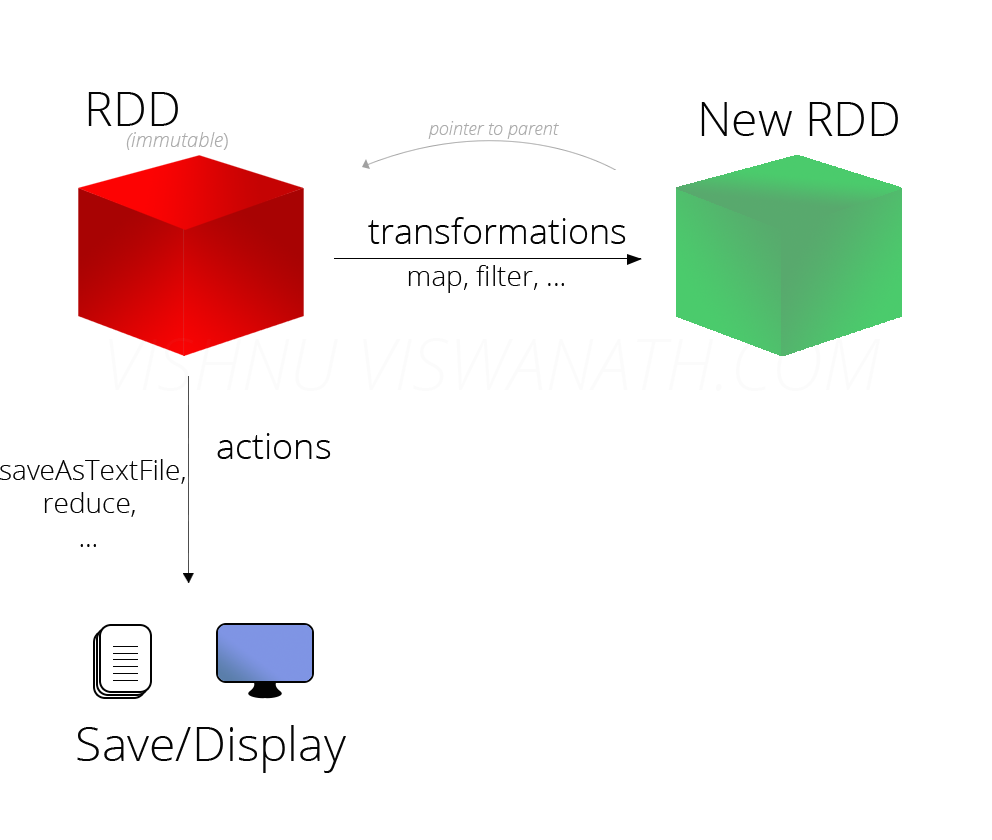
\includegraphics[width=\textwidth,height=6.5cm]{Graphics/Actions_Transformations.png}
		\end{figure}
\end{frame}


%%%%%%%%%%%%%%%%%%%%%%%%%%%%%%%%%%%%%%%%%%%%%%%%%%%%%%%%%%%%%%%%%%%%%%%%%%%
%
%
%
%%%%%%%%%%%%%%%%%%%%%%%%%%%%%%%%%%%%%%%%%%%%%%%%%%%%%%%%%%%%%%%%%%%%%%%%%%%

\subsubsection{Transformations}
\begin{frame}
  \frametitle{RDD Operations: Transformations(1/2)}
	\begin{itemize}[<+->]
		\item Transformations create a new RDD from an exising one
		\item It works on one element at a time; but this is not true for all transformations
		\item \textbf{RDDs are immutable}
			\begin{itemize}
			\item Data in an RDD is never changed
			\item Transform in sequence to modify the data as needed
			\item If we want to make any edit in the dataset you need to transform and the output of transformation will be save into new dataset
			\item How can Spark know if we have multi-stages? 
			\item Spark keep track of each step you transform the data into \\ \textbf{lineage graph} 
			\end{itemize}
	\end{itemize}
\end{frame}


%%%%%%%%%%%%%%%%%%%%%%%%%%%%%%%%%%%%%%%%%%%%%%%%%%%%%%%%%%%%%%%%%%%%%%%%%%%
\begin{frame}
  \frametitle{RDD Operations: Transformations(2/2)}

%TCIDATA%to add caption RDD lineage graph
  \begin{figure}
	\caption{Example how filter/map transformation work}  	
		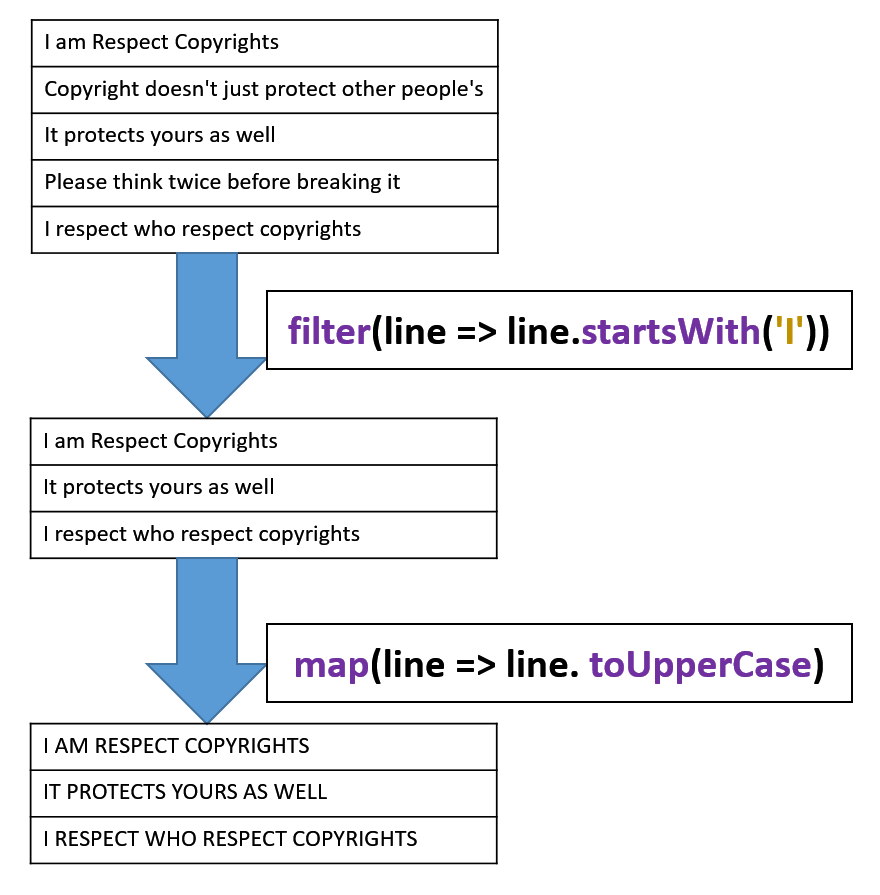
\includegraphics[width=\textwidth,height=6.5cm]{Graphics/MapGraph.PNG}
\end{figure}

%TCIDATA%To add Examples here to illistruate the idea of split index

%TCIDATA to create a seprate section for this part
\end{frame}

%%%%%%%%%%%%%%%%%%%%%%%%%%%%%%%%%%%%%%%%%%%%%%%%%%%%%%%%%%%%%%%%%%%%%%%%%%%
%
%
%
%%%%%%%%%%%%%%%%%%%%%%%%%%%%%%%%%%%%%%%%%%%%%%%%%%%%%%%%%%%%%%%%%%%%%%%%%%%




\subsubsection{Actions}

\begin{frame}[fragile]
  \frametitle{RDD Operations: Actions(1/4)}
	\begin{itemize}[<+->]
%TCIDATA to define a new type of defnintion it is name semi definition
		\item They are the operations that return a final value to the driver program or write data to an external storage system
		\item Actions force the evaluation of the transformations required for the RDD they were called on
	\end{itemize}
\end{frame}

\begin{frame}[fragile]
	\frametitle{RDD Operations: Actions(2/4)}

		\begin{lstlisting}[style=myScalastyle, caption=RDD Actions Example 2]
		//print first 10 line from filtered data RDD 
		//note tjat you can remove the foreach println if you are working in shell but if you will use scala in you external job you need to add it.
		scala> filter_lines.take(10).foreach(println)
		"high-level APIs in Scala, Java, Python, and R, and an optimized engine that"
		## Interactive Scala Shell
		The easiest way to start using Spark is through the Scala shell:
		\end{lstlisting}
\end{frame}


\begin{frame}
  \frametitle{RDD Operations: Actions(3/4)}
	\begin{itemize}[<+->]
		\item What actual happen when you do any action?
		\begin{itemize}
			\item The data will be retrieved to the driver program
			\item you can use collect to retrieve the all entire dataset,But Please don't use it unless the data is very small
			\item Keep in mind that your entire dataset must fit in memory on a single machine to use collect\(\)
			\item Also keep in mind again "Sorry to keep a lot of info into your mind " \\ the entire RDD must be computed “from scratch.” it is very costly to reprocess my data from scratch
			\item We need to find a way to save the intermediate results into somewhere but please try to keep it in-memory. "Will be discussed later small hint '\textit{persist or cashe}' "
		\end{itemize}
	\end{itemize}
\end{frame}

\begin{frame}
  \frametitle{RDD Operations: Actions(4/4)}
 	\begin{itemize}[<+->]
		\item What I should do to do actions on the full data in Large datasets? 
		\begin{itemize}
			\item It’s common to write data out to a distributed storage system such as HDFS or Amazon S3
			\item You can save the contents of an RDD using the saveAsTextFile\(\) \\ action, saveAsSequenceFile\(\)
			\item Keep in mind that your entire dataset must fit in memory on a single machine to use collect\(\)
			%TCIDATA Is the driver is only single machine
		\end{itemize}
	\end{itemize}
\end{frame}
% How spark really run our jobs in distributed mode and what is the concepts of the parallel and how it works?

%%%%%%%%%%%%%%%%%%%%%%%%%%%%%%%%%%%%%%%%%%%%%%%%%%%%%%%%%%%%%%%%%%%%%%%%%%%

			%TCIDATA Use Scala or python into huge projects   --------- to be Added


			%TCIDATA check if we can highlighted some keywords into normal  latex text    --------- to be Added

			%TCIDATA Is the driver is only single machine
%%%%%%%%%%%%%%%%%%%%%%%%%%%%%%%%%%%%%%%%%%%%%%%%%%%%%%%%%%%%%%%%%%%%%%%%%%%
%
%
%
%%%%%%%%%%%%%%%%%%%%%%%%%%%%%%%%%%%%%%%%%%%%%%%%%%%%%%%%%%%%%%%%%%%%%%%%%%%

\subsection{Functional programming features}
\begin{frame}
  \frametitle{Functional programming features}
 	\begin{itemize}[<+->]
		\item As we know spark core implementation built on scala. So, it must have some features these features inherited from Functional programming concepts not Spark. Then spark team implement the transformation to be distributed
	\end{itemize}
\end{frame}

%%%%%%%%%%%%%%%%%%%%%%%%%%%%%%%%%%%%%%%%%%%%%%%%%%%%%%%%%%%%%%%%%%%%%%%%%%%
%
%
%
%%%%%%%%%%%%%%%%%%%%%%%%%%%%%%%%%%%%%%%%%%%%%%%%%%%%%%%%%%%%%%%%%%%%%%%%%%%

\subsubsection{Lazy Evaluation}

\begin{frame}[fragile]
	  \frametitle{Lazy Evaluation (1/4)}
\begin{itemize}[<+->]
			\begin{lstlisting}[style=myScalastyle, caption=Spark Lazy Execution Example]
scala> val input = sc.parallelize(List("Mostafa Alaa,Big Data,Etisalat,Smart Cities Project"))
res: input: org.apache.spark.rdd.RDD[String] = ParallelCollectionRDD[6] at parallelize at <console>:24
scala> val splittedCommaMap = input.map(x => x.split(","))
res2: splittedCommaMap: org.apache.spark.rdd.RDD[Array[String]] = MapPartitionsRDD[8]	
scala> inputMapped.collect.map(x => x.foreach(println))
res3: Array[Unit] = Array(())
"Mostafa Alaa"
"Big Data"
"Etisalat"
"Smart Cities Project"
			\end{lstlisting}

\end{itemize}
\end{frame}


\begin{frame}
	  \frametitle{Lazy Evaluation (2/4)}
\begin{itemize}[<+->]
	\item What if we pass a string to map and split on index 3 and the string has two index only?
	\item Does spark evaluate our transformation once we do mapping ?
\end{itemize}
\end{frame}

\begin{frame}
	  \frametitle{Lazy Evaluation (3/4)}
	    \begin{figure}
	  	\caption{Lazy Evaluation Execution 1}  
	  			  	
			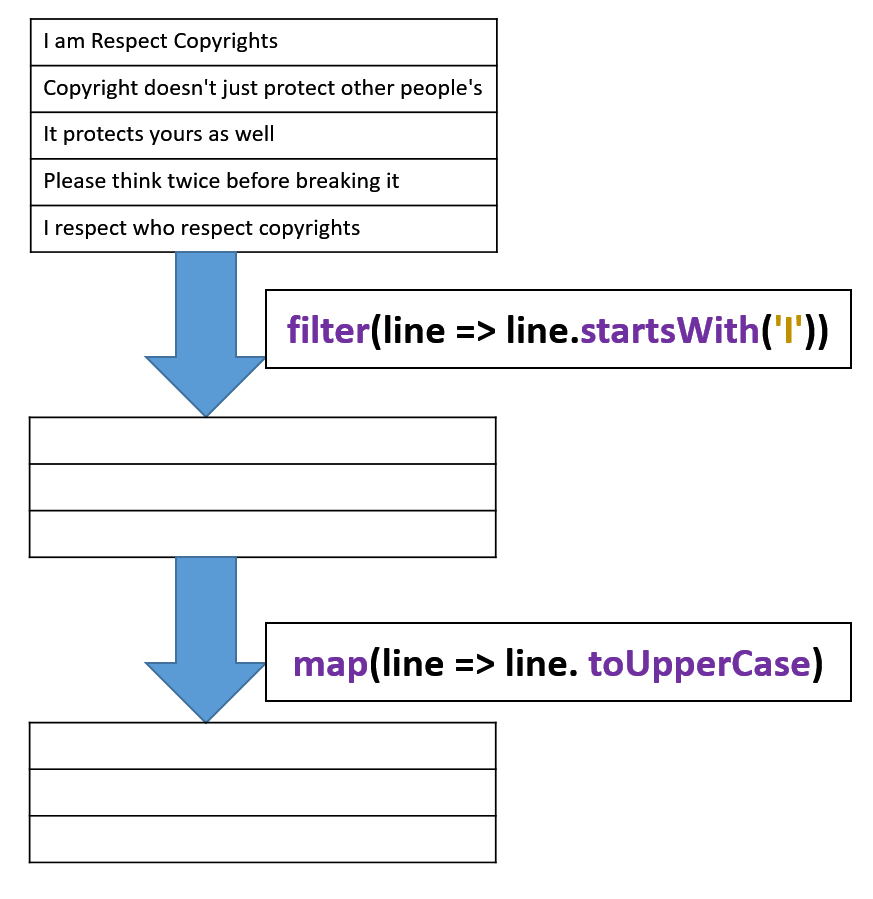
\includegraphics[width=\textwidth,height=6.5cm]{Graphics/lazy1.PNG}
		\end{figure}
\end{frame}

\begin{frame}
	  \frametitle{Lazy Evaluation (4/4)}
	    \begin{figure}
	  	\caption{Lazy Evaluation Execution 2}  
			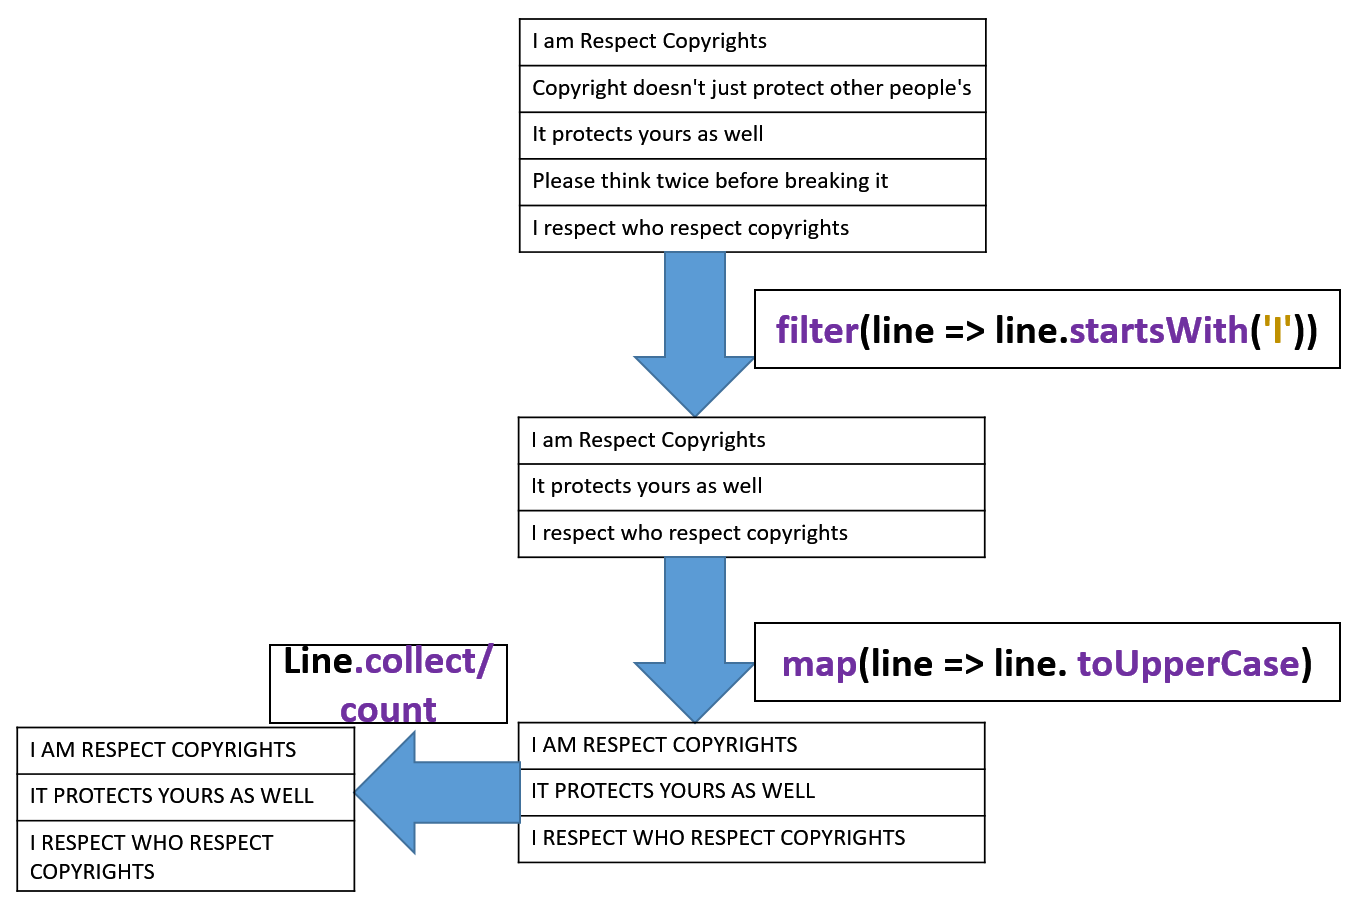
\includegraphics[width=\textwidth,height=6.5cm]{Graphics/lazy2.PNG}
		\end{figure}
\end{frame}

%%%%%%%%%%%%%%%%%%%%%%%%%%%%%%%%%%%%%%%%%%%%%%%%%%%%%%%%%%%%%%%%%%%%%%%%%%%
%
%
%
%%%%%%%%%%%%%%%%%%%%%%%%%%%%%%%%%%%%%%%%%%%%%%%%%%%%%%%%%%%%%%%%%%%%%%%%%%%


\subsubsection{Chaining Transformations}
\begin{frame}
	  \frametitle{Chaining Transformations (1/2)}
	    \begin{figure}
	  	\caption{Chaining Transformations}  		  	
			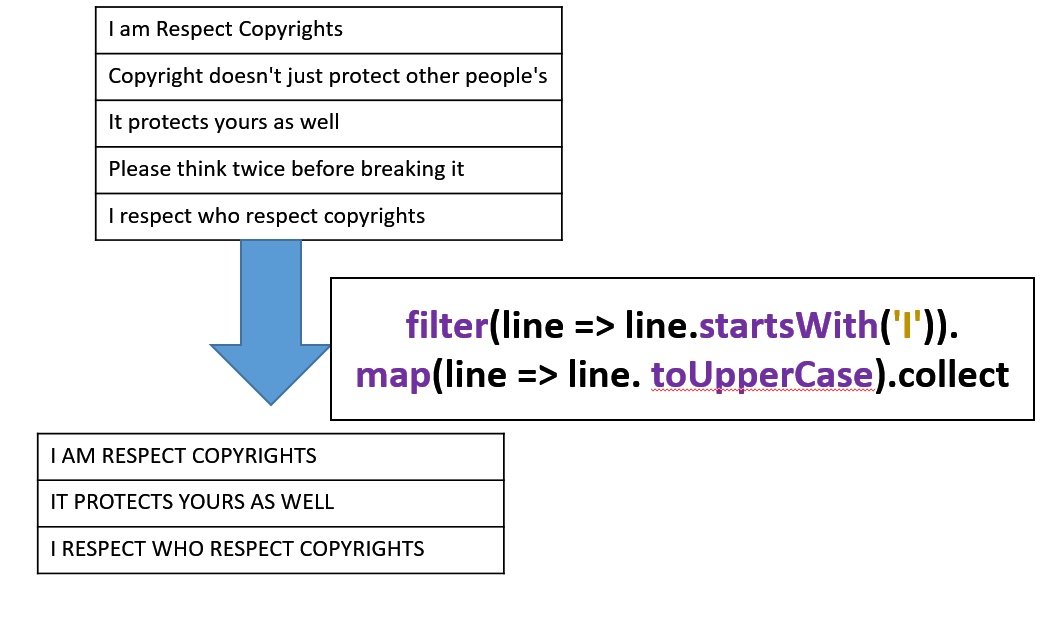
\includegraphics[width=\textwidth]{Graphics/chain.PNG}
		\end{figure}
	
\end{frame}


\begin{frame}[fragile]
	  \frametitle{Chaining Transformations (2/2)}

			\begin{lstlisting}[style=myScalastyle, caption=Chaining Transformations Execution Example]

scala> val lines = sc.textFile("README.md")
scala> lines.take(3)
				
// is the same as 
val lines = sc.textFile("README.md").take(3)
			\end{lstlisting}
\begin{itemize}[<+->]

\item How Spark work with both? please check this function and you will got it "toDebugString"
\end{itemize}
\end{frame}

%%%%%%%%%%%%%%%%%%%%%%%%%%%%%%%%%%%%%%%%%%%%%%%%%%%%%%%%%%%%%%%%%%%%%%%%%%%
%
%
%
%%%%%%%%%%%%%%%%%%%%%%%%%%%%%%%%%%%%%%%%%%%%%%%%%%%%%%%%%%%%%%%%%%%%%%%%%%%

\subsubsection{Pipelining}
\begin{frame}
	  \frametitle{Pipelining (1/3)}
		\begin{itemize}[<+->]
			\item Motivation question: If you have huge amounts of data and you need to print sample of this data Ex: 3, what spark will do?
		\end{itemize}
\end{frame}

\begin{frame}
	  \frametitle{Pipelining (2/3)}
	    \begin{figure}
	  	\caption{Pipelining Example Part 1}  		  	
			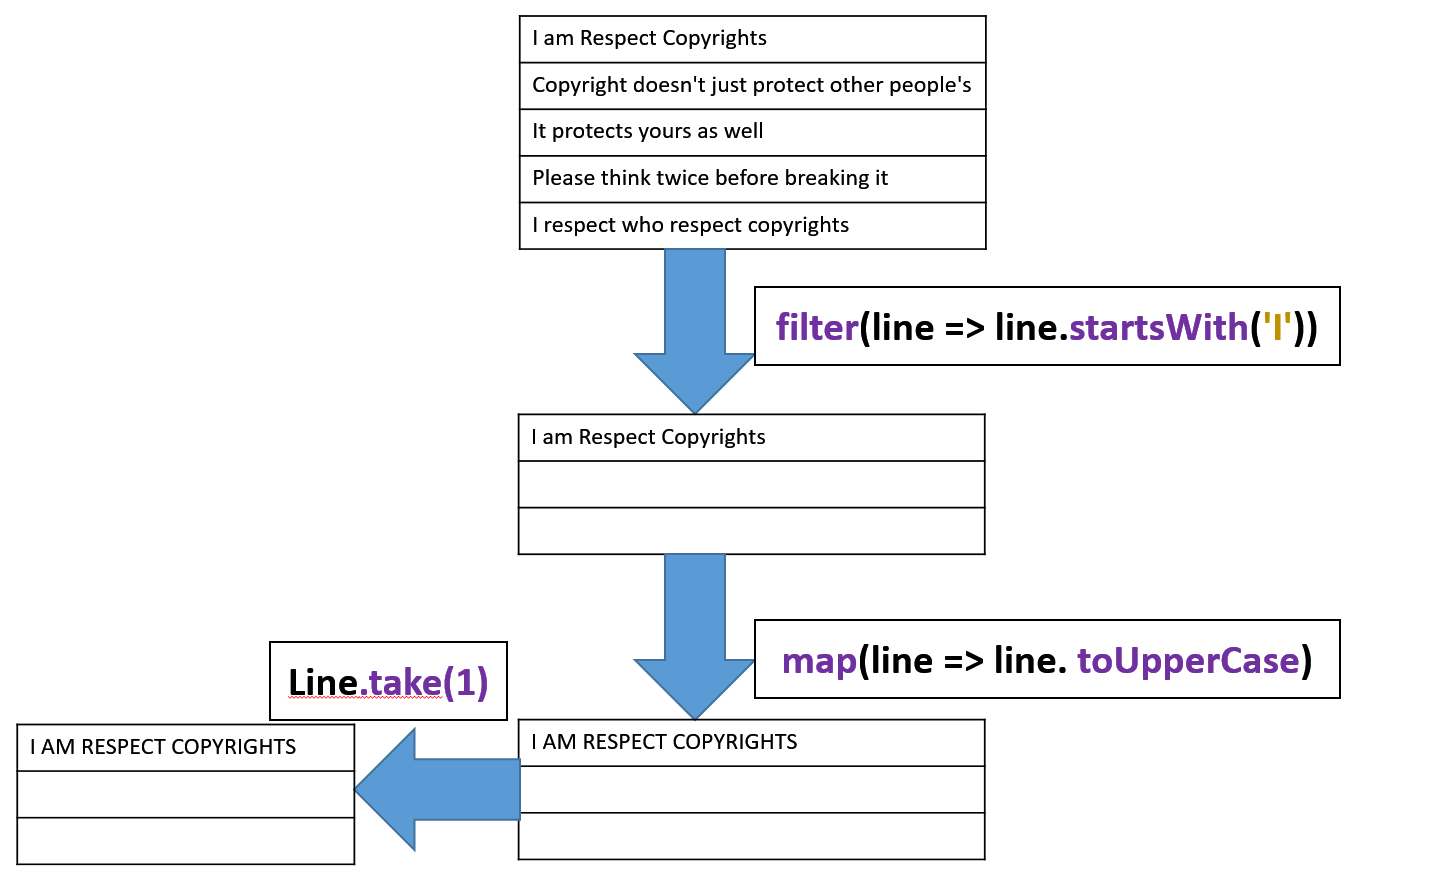
\includegraphics[width=\textwidth,height=6.5cm]{Graphics/take1pipe.PNG}
		\end{figure}
\end{frame}

\begin{frame}
	  \frametitle{Pipelining (3/3)}
	    \begin{figure}
	  	\caption{Pipelining Example Part 2}  		  				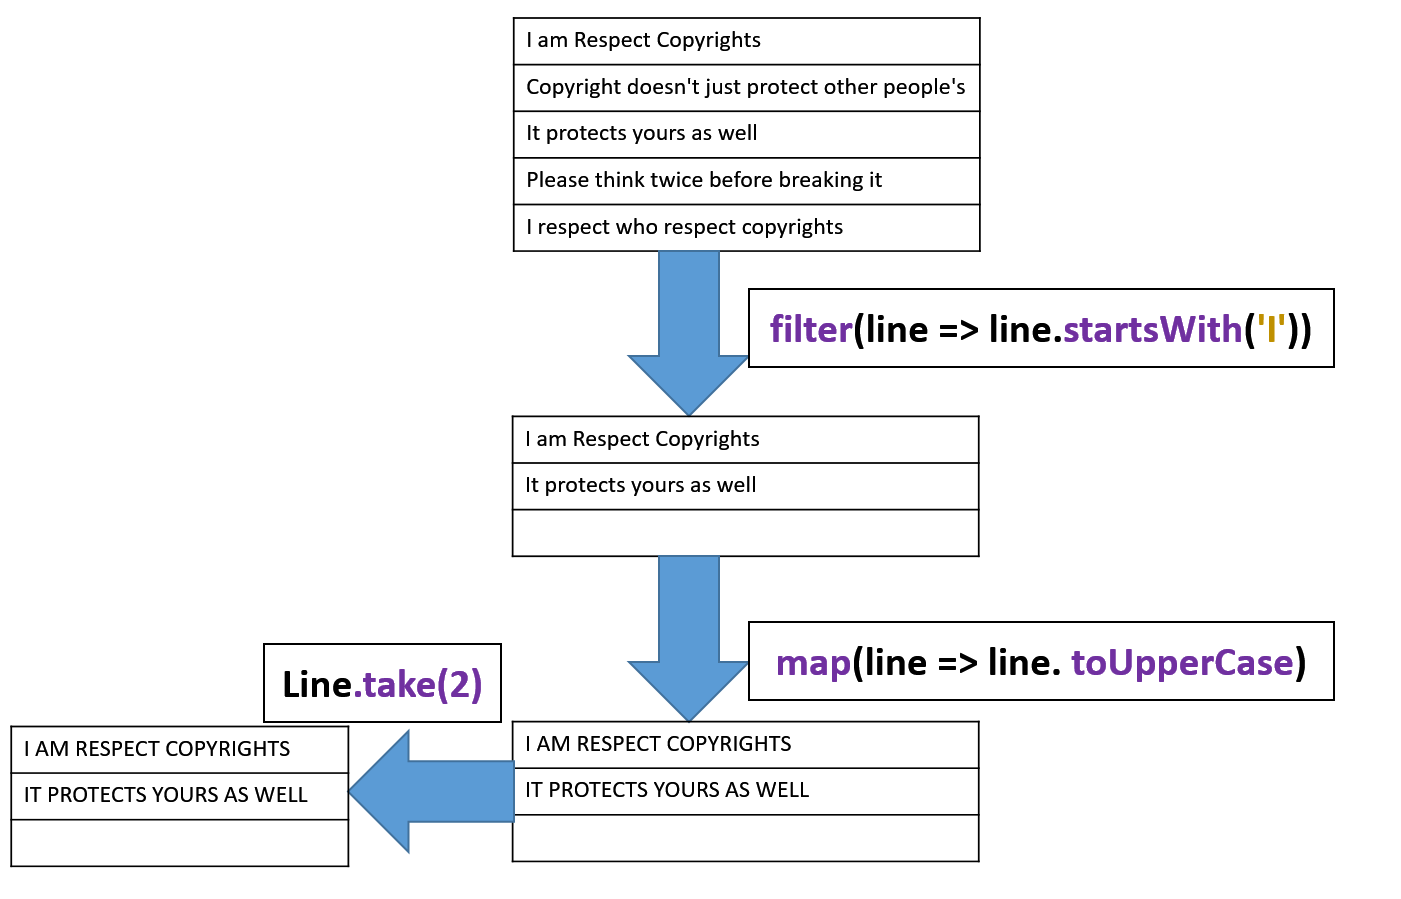
\includegraphics[width=\textwidth,height=6.5cm]{Graphics/take2pipe.PNG}
		\end{figure}
\end{frame}
%%%%%%%%%%%%%%%%%%%%%%%%%%%%%%%%%%%%%%%%%%%%%%%%%%%%%%%%%%%%%%%%%%%%%%%%%%%
%
%
%
%%%%%%%%%%%%%%%%%%%%%%%%%%%%%%%%%%%%%%%%%%%%%%%%%%%%%%%%%%%%%%%%%%%%%%%%%%%



\subsubsection{Passing Functions to Spark}
\begin{frame}[fragile]
	  \frametitle{Passing Functions to Spark}
\begin{itemize}[<+->]
\item Spark depends heavily on the concepts of functional programming
\item Functions are the fundamental unit of programming
\item You need to think you will have a function passed to another function
\item Most of modern programming language has the concept of anonymous functions
\end{itemize}
			\begin{lstlisting}[style=myScalastyle, caption=Passing Functions to RDD Example]

def chnageString(s: String): String =
{ s +"AAA" }				
				
//Lets show our Data using "Take"
scala> lines.map(chnageString).take(2)
			
			\end{lstlisting}
\end{frame}
%%%%%%%%%%%%%%%%%%%%%%%%%%%%%%%%%%%%%%%%%%%%%%%%%%%%%%%%%%%%%%%%%%%%%%%%%%%
%
%
%
%%%%%%%%%%%%%%%%%%%%%%%%%%%%%%%%%%%%%%%%%%%%%%%%%%%%%%%%%%%%%%%%%%%%%%%%%%%

\subsection{Persistence (Caching)}
\begin{frame}[fragile]
	  \frametitle{Persistence (Caching) (1/11)}
\begin{itemize}[<+->]
\item Spark RDDs are lazily evaluated, and sometimes we may wish to use the same RDD multiple times
\item Spark will recompute the RDD and all of its dependencies each time we call an action on the RDD
\item This can be especially expensive for iterative algorithms
	\begin{lstlisting}[style=myScalastyle, caption=Motivation Example Persistence]
val result = input.map(x => x*x)
println(result.count())
println(result.collect().mkString(","))
	\end{lstlisting}
\end{itemize}
\end{frame}


\begin{frame}[fragile]
	\frametitle{Persistence (Caching) (2/11)}
	\begin{itemize}[<+->]

\item What will happened if one of the nodes that has data persisted failed? \textit{spark will recompute the lost partitions of the data when needed}

\item How to avoid the cost of recompute the data? \textit{We can also replicate our data on multiple nodes if we want to be able to handle node failure without slowdown}


\end{itemize}
\end{frame}

\begin{frame}
	  \frametitle{Persistence (Caching) (3/11)}
	    \begin{figure}
	  	\caption{Spark Caching Example Part 1}  		  	
			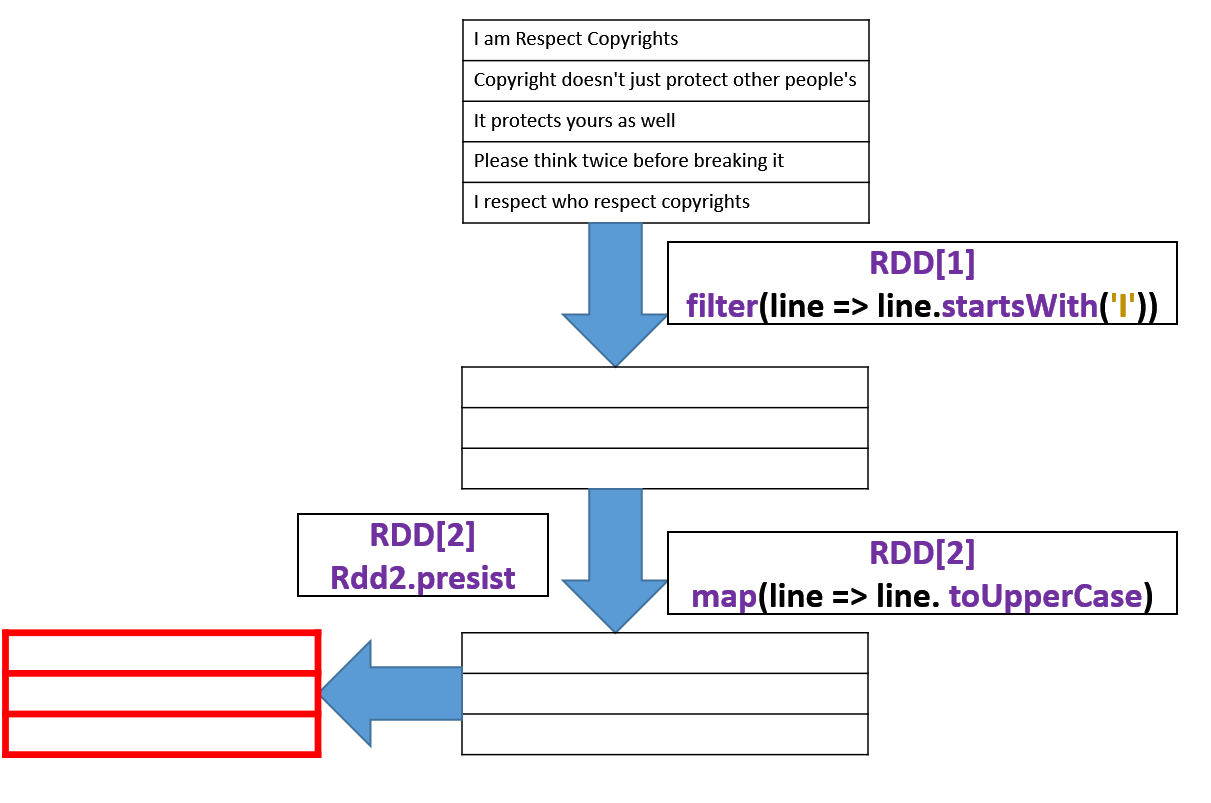
\includegraphics[width=\textwidth,height=6.5 cm]{Graphics/cashe1.PNG}
		\end{figure}
\end{frame}

\begin{frame}
	  \frametitle{Persistence (Caching) (4/11)}
	    \begin{figure}
	  	\caption{Spark Caching Example Part 2}  		  	
			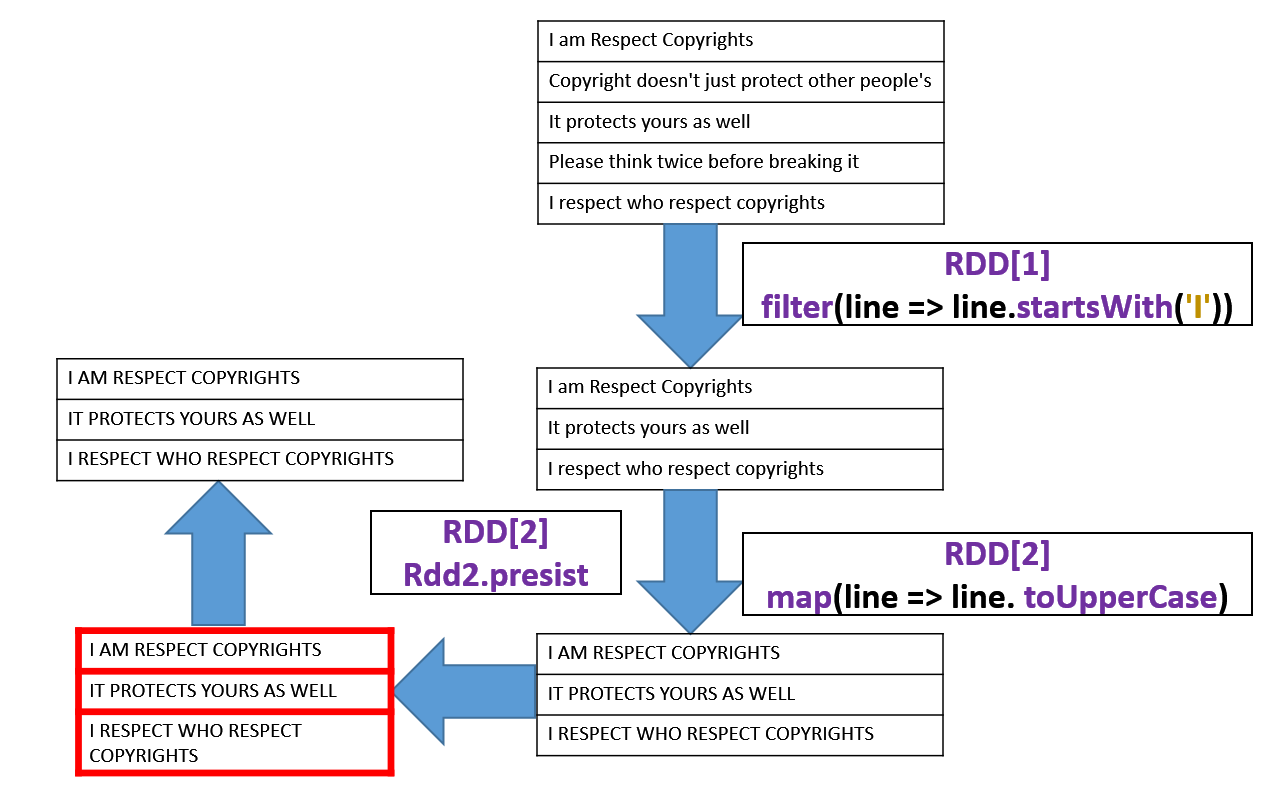
\includegraphics[width=\textwidth,height=6.5cm]{Graphics/cashe2.PNG}
		\end{figure}
\end{frame}

\begin{frame}[fragile]
	  \frametitle{Persistence (Caching) (5/11)}
	\begin{itemize}[<+->]
		\item You control storage (location,format in memory, partition replication)
			\begin{itemize}
				\item MEMORY\_ONLY(default)
				\item MEMORY\_AND\_DISK
				\item DISK\_ONLY
			\end{itemize}
	\end{itemize}
		\begin{lstlisting}[style=myScalastyle, caption=Persistence Storage Level Example]
import org.apache.spark.storage.StorageLevel
data.persist(StorageLevel.MEMORY_AND_DISK.)
		\end{lstlisting}
\end{frame}


\begin{frame}
	  \frametitle{Persistence (Caching) (6/11)}
	\begin{itemize}[<+->]
		\item Serialization
			\begin{enumerate}
			\item MEMORY\_ONLY\_SER
			\item MEMORY\_AND\_DISK\_SER
			\end{enumerate}
		\item Partition replication –store partitions on two nodes
			\begin{enumerate}
			\item MEMORY\_ONLY\_2
			\item MEMORY\_AND\_DISK\_2
			\item DISK\_ONLY\_2
			\item MEMORY\_ONLY\_SER\_2
			\item MEMORY\_AND\_DISK\_SER\_2
			\end{enumerate}

	\end{itemize}
\end{frame}

\begin{frame}
	\frametitle{Persistence (Caching) (7/11)}
	\begin{itemize}[<+->]
		\item spark cache vs persist
		\begin{enumerate}
			\item The difference between cache and persist operations is purely syntactic. cache is a synonym of persist or persist(MEMORY\_ONLY), i.e. cache is merely persist with the default storage level MEMORY\_ONLY
			\item you can cache a RDD in memory doesn’t mean you should blindly do so. Depending on how many times the dataset is accessed and the amount of work involved in doing so, re-computation can be faster than the price paid by the increased memory pressure
		\end{enumerate}
		
	\end{itemize}
\end{frame}

\begin{frame}
	\frametitle{Persistence (Caching) (8/11)}
	  \begin{figure}
			\caption{Spark Program Workflow By RDD}  		  	
			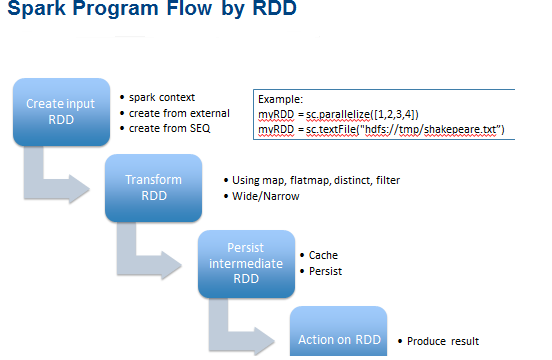
\includegraphics[width=\textwidth,height=6.5cm]{Graphics/SparkWF.PNG}
		\end{figure}
		
\end{frame}


\begin{frame}
	\frametitle{Persistence (Caching) (9/11)}
		\begin{figure}
			\caption{Cache in memory}  		  	
			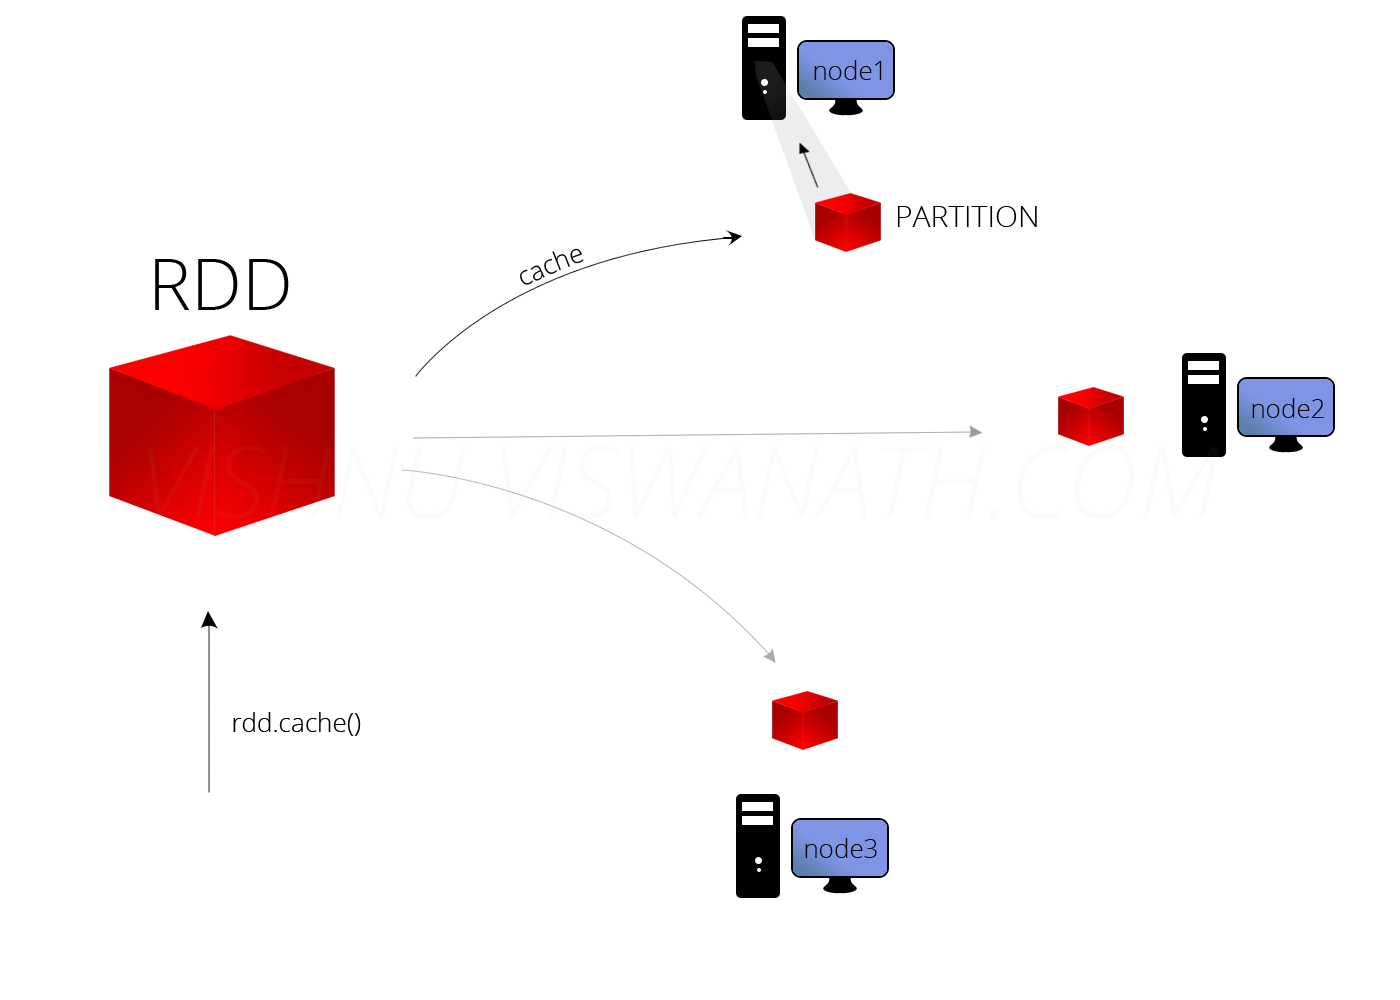
\includegraphics[width=\textwidth,height=6.5cm]{Graphics/cache.png}
		\end{figure}
\end{frame}


\begin{frame}
	\frametitle{Persistence (Caching) (10/11)}
		\begin{figure}
			\caption{Persist in memory and disk}  		  	
			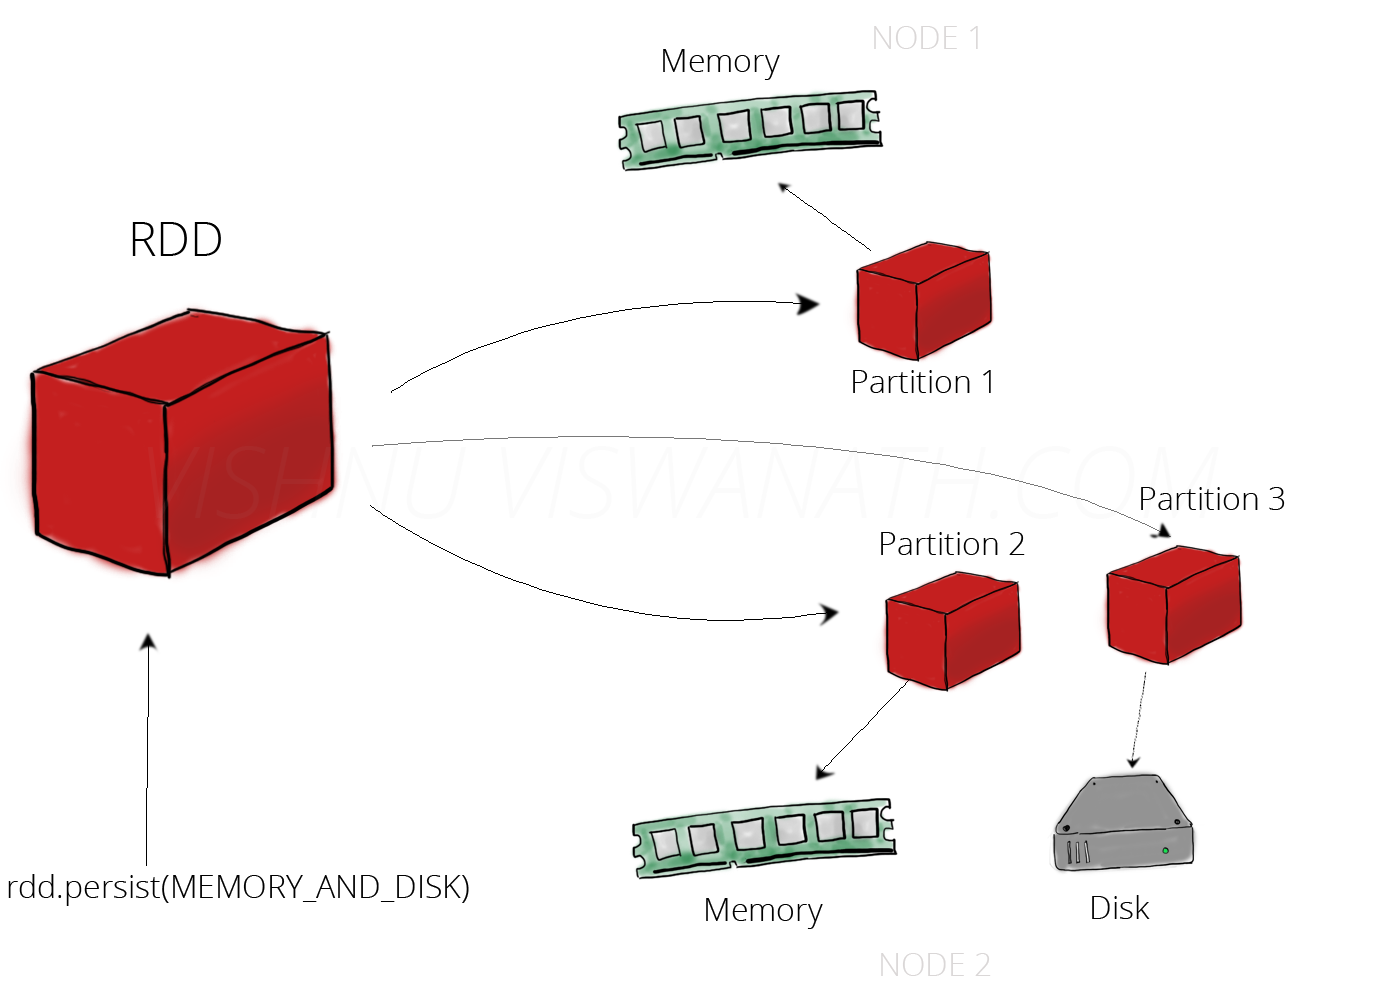
\includegraphics[width=\textwidth,height=6.5cm]{Graphics/persist.PNG}
		\end{figure}
		
\end{frame}



\begin{frame}
	\frametitle{Persistence (Caching) (11/11)}
	\begin{itemize}[<+->]
		\item Recommendations
		\begin{enumerate}
			\item Use persist (memory and disk) when you are not sure the amount of data
			\item Use persist/cache whenever you have dataset which has huge computation dependency
			\item You need to use the Spark cache/persist to take the advantage of computation speed but take care
		\end{enumerate}
	\end{itemize}
\end{frame}

\subsection{Broadcast variables}

\begin{frame}[fragile]
	\frametitle{Broadcast variables (1/6)}
	\begin{itemize}[<+->]
		\item A broadcast variable, is a type of shared variable, used for broadcasting data across the cluster
		\item Hadoop MapReduce users can relate this to distributed cache
			\begin{lstlisting}[style=myScalastyle, caption=Broadcast variables Example]

val names = sc.textFile("/names").map(line => (line.split(",")(3),line))
val addresses = sc.textFile("/address").map(line => (line.split(",")(0),line))
names.join(addresses)
\end{lstlisting}
		\item Here, both names and addresses will be shuffled over the network for performing the join which is not efficient since any data transfer over the network will reduce the execution speed
	\end{itemize}
\end{frame}

\begin{frame}
	\frametitle{Broadcast variables (2/6)}
		\begin{figure}
			\caption{Broadcast variables Shuffle over Network}  		  	
			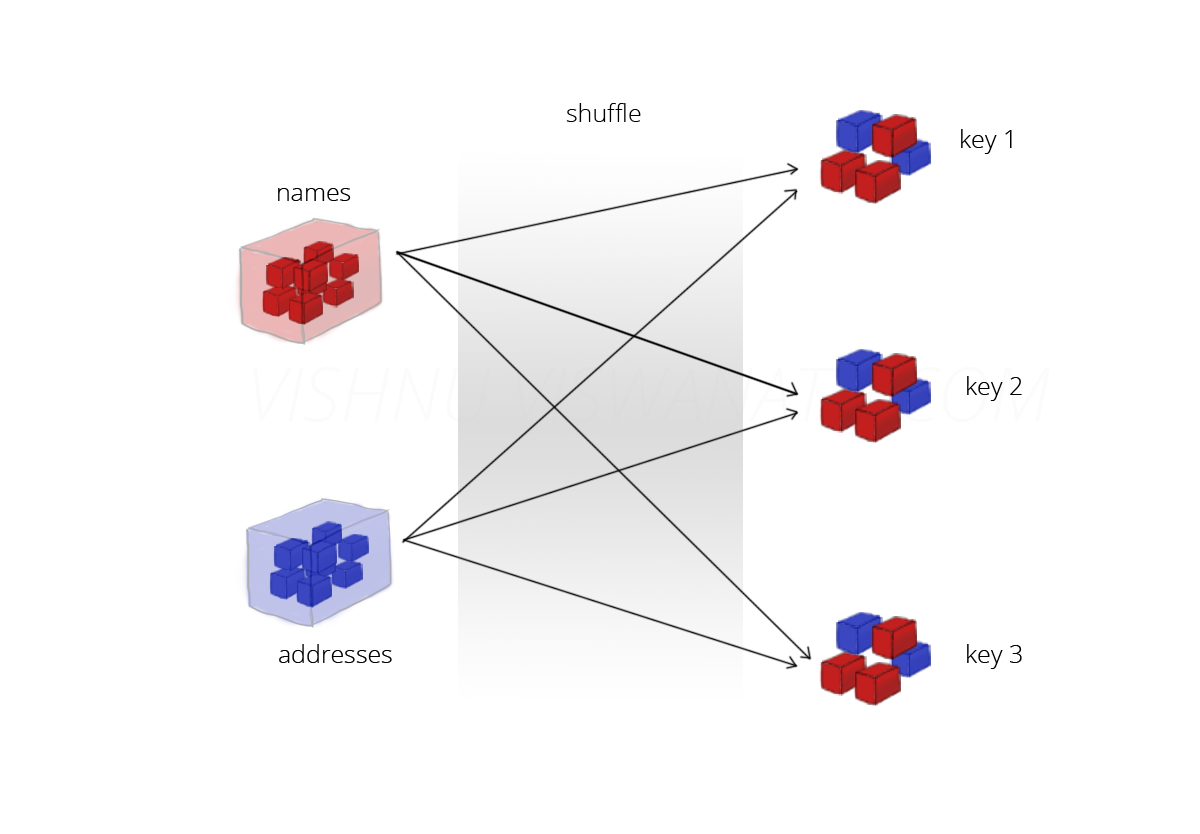
\includegraphics[width=\textwidth,height=6.5cm]{Graphics/Broadcastvariables.png}
		\end{figure}

\end{frame}



\begin{frame}[fragile]
	\frametitle{Broadcast variables (3/6)}
	\begin{itemize}[<+->]
		\item Another approach is, if one of the RDDs is small in size, we can choose to send it to each node only once, thereby reducing network traffic
		\item \textbf{Note that:} Broadcast variables are read-only, broadcast.value is an immutable object
		along with each task. Consider the below example
		\begin{lstlisting}[style=myScalastyle, caption=Broadcast variables Enhanced Example]
		
		val names = sc.textFile("/names").map(line => (line.split(",")(3),line))
		val addresses = sc.textFile("/address").map(line => (line.split(",")(0),line))
		val addressedMap = addresses.collect().toMap
		val broadcast = sc.broadcast(addressedMap)
		val joined =  names.map(v => v._2,(broadcast.value(v._1)))
		\end{lstlisting}		
	\end{itemize}
\end{frame}

\begin{frame}
	\frametitle{Broadcast variables (4/6)}
	\begin{figure}
		\caption{Join using Broadcast variables}	
		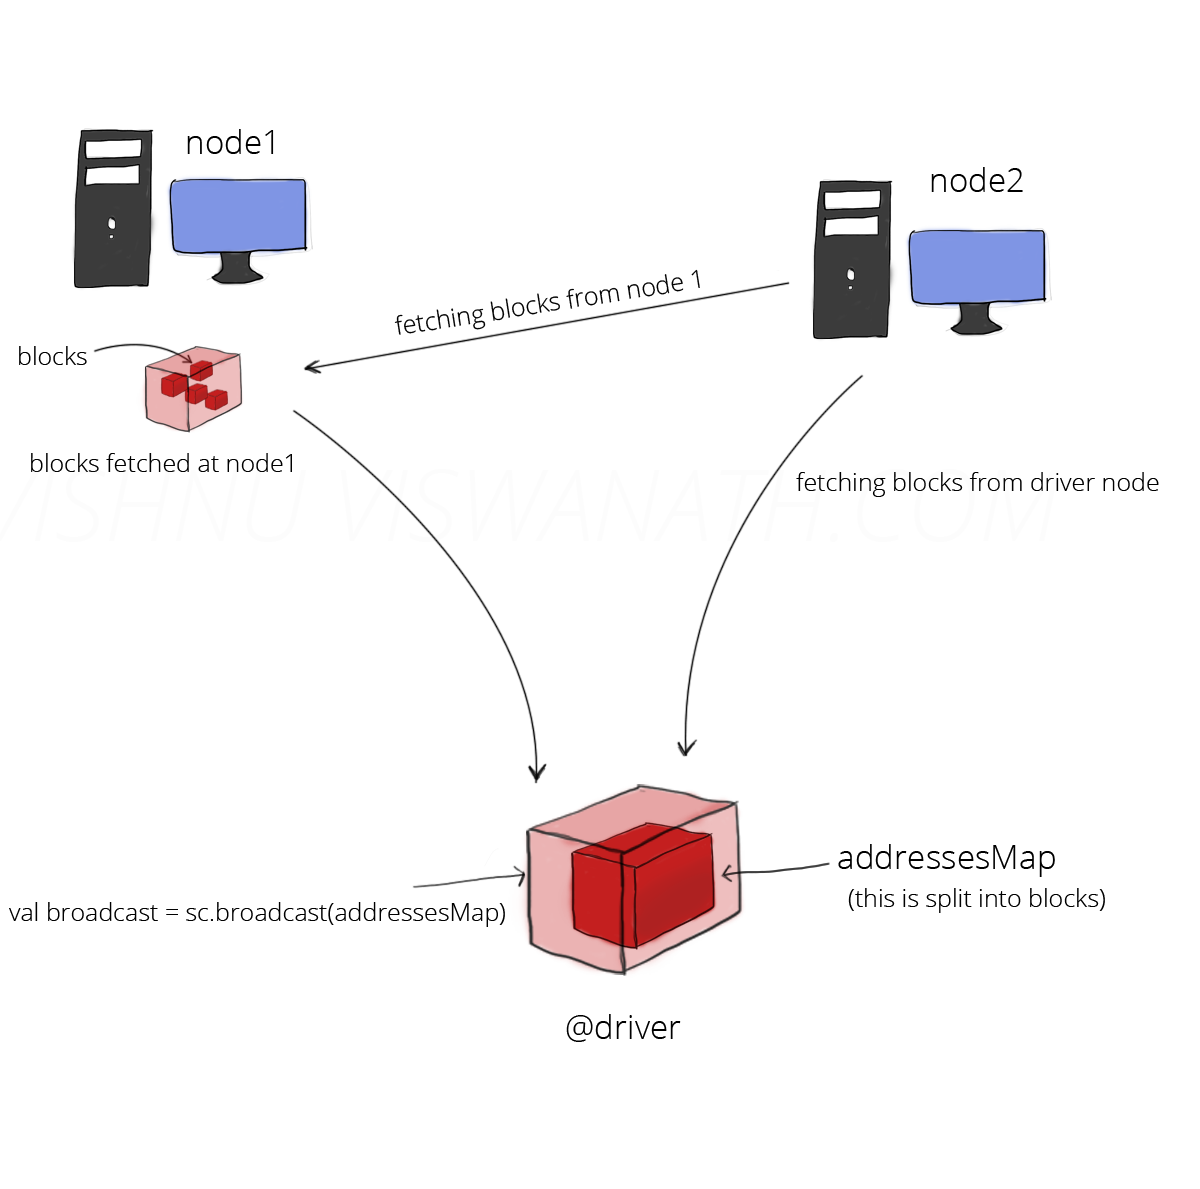
\includegraphics[width=\textwidth,height=6.5cm]{Graphics/BitTorrent.png}
	\end{figure}
	
\end{frame}



\begin{frame}
	\frametitle{Broadcast variables (5/6)}
	\begin{itemize}[<+->]
		\item Spark uses BitTorrent like protocol for sending the broadcast variable across the cluster, i.e., for each variable that has to be broadcasted, initially the driver will act as the only source. The data will be split into blocks at the driver and each leecher (receiver) will start fetching the block to it’s local directory
		\item Once a block is completely received, then that leecher will also act as a source for this block for the rest of the leechers (This reduces the load at the machine running driver).

	\end{itemize}
\end{frame}


\begin{frame}
	\frametitle{Broadcast variables (6/6)}
	\begin{itemize}[<+->]
		\item This is continued for rest of the blocks. So initially, only the driver is the source and later on the number of sources increases – because of this, rate at which the blocks are fetched by a node increases over time
		\item \textbf{Note that:} We are talking about small lookups not huge amount of data. If you are using it with huge tables that will joined so, Job will be failed easily. 
		along with each task.
	\end{itemize}
\end{frame}


%%%%%%%%%%%%%%%%%%%%%%%%%%%%%%%%%%%%%%%%%%%%%%%%%%%%%%%%%%%%%%%%%%%%%%%%%%%
%
%
%
%%%%%%%%%%%%%%%%%%%%%%%%%%%%%%%%%%%%%%%%%%%%%%%%%%%%%%%%%%%%%%%%%%%%%%%%%%%

\subsection{Questions about spark engine}
\begin{frame}
	  \frametitle{Questions about spark engine}
	\begin{itemize}[<+->]
		%to define Engin Questions here !!!!!!!
		\item Tricky question: where spark save the linage? and what if linage lost?
		\item If we apply the transformation then spark will execute the datasets and get the results?
		\item Does map,filter and other functions is spark function at the beginning? 
		\item Does spark main language which built on scala affect the thinking of the developers who develop spark?
		\item Transformation is only the spark built functions?
		\item Can we define a function and apply it to the a data? or we are limited with spark defined functions?
	\end{itemize}
\end{frame}

%%%%%%%%%%%%%%%%%%%%%%%%%%%%%%%%%%%%%%%%%%%%%%%%%%%%%%%%%%%%%%%%%%%%%%%%%%%
%
%
%
%%%%%%%%%%%%%%%%%%%%%%%%%%%%%%%%%%%%%%%%%%%%%%%%%%%%%%%%%%%%%%%%%%%%%%%%%%%


%
%\subsection{Accumulators}
%	  \frametitle{Accumulators (1/2)}
%\begin{itemize}[<+->]
%	%to define Engin Questions here !!!!!!!
%	\item Accumulators, as the name suggests accumulates data during execution. This is similar to Counters in Hadoop MapReduce.
%	\item An accumulator is initialized at the driver and is then modified(added) by each executor. Finally, all these values are aggregated back at the driver.
%	
%\end{itemize}
%
%
%
%\begin{frame}[fragile]
%	\frametitle{Accumulators (2/2)}
%		\begin{lstlisting}[style=myScalastyle, caption=Accumulators Example]
%		
%		val names = sc.textFile("/names").map(line => (line.split(",")(3),line))
%		val addresses = sc.textFile("/address").map(line => (line.split(",")(0),line))
%		val addressedMap = addresses.collect().toMap
%		val broadcast = sc.broadcast(addressedMap)
%		val joined =  names.map(v => v._2,(broadcast.value(v._1)))
%		
%		val accum = sc.accumulator(0,"india_counter")
%		joined.foreach(v => if(v._2.contains("india")) accum +1)
%		\end{lstlisting}		
%\end{frame}






%%%%%%%%%%%%%%%%%%%%%%%%%%%%%%%%%%%%%%%%%%%%%%%%%%%%%%%%%%%%%%%%%%%%%%%%%%%
%
%
%
%%%%%%%%%%%%%%%%%%%%%%%%%%%%%%%%%%%%%%%%%%%%%%%%%%%%%%%%%%%%%%%%%%%%%%%%%%%

%\section{Working with Key/Value Pairs}
%\begin{frame}
%	  \frametitle{Working with Key/Value Pairs}
%\end{frame}
%
%\subsection{Motivation}
%\begin{frame}
%	  \frametitle{Working with Key/Value Pairs}
%\end{frame}
%%%%%%%%%%%%%%%%%%%%%%%%%%%%%%%%%%%%%%%%%%%%%%%%%%%%%%%%%%%%%%%%%%%%%%%%%%%%
%%
%%
%%
%%%%%%%%%%%%%%%%%%%%%%%%%%%%%%%%%%%%%%%%%%%%%%%%%%%%%%%%%%%%%%%%%%%%%%%%%%%%
%
%\subsection{Creating Pair RDDs}
%\begin{frame}
%	  \frametitle{Working with Key/Value Pairs}
%\end{frame}
%%%%%%%%%%%%%%%%%%%%%%%%%%%%%%%%%%%%%%%%%%%%%%%%%%%%%%%%%%%%%%%%%%%%%%%%%%%%
%%
%%
%%
%%%%%%%%%%%%%%%%%%%%%%%%%%%%%%%%%%%%%%%%%%%%%%%%%%%%%%%%%%%%%%%%%%%%%%%%%%%%
%
%
%\subsection{Transformations on Pair RDDs}
%\begin{frame}
%	  \frametitle{Working with Key/Value Pairs}
%\end{frame}
%%%%%%%%%%%%%%%%%%%%%%%%%%%%%%%%%%%%%%%%%%%%%%%%%%%%%%%%%%%%%%%%%%%%%%%%%%%%
%%
%%
%%
%%%%%%%%%%%%%%%%%%%%%%%%%%%%%%%%%%%%%%%%%%%%%%%%%%%%%%%%%%%%%%%%%%%%%%%%%%%%
%
%\subsection{Aggregations}
%\begin{frame}
%	  \frametitle{Working with Key/Value Pairs}
%\end{frame}
%%%%%%%%%%%%%%%%%%%%%%%%%%%%%%%%%%%%%%%%%%%%%%%%%%%%%%%%%%%%%%%%%%%%%%%%%%%%
%%
%%
%%
%%%%%%%%%%%%%%%%%%%%%%%%%%%%%%%%%%%%%%%%%%%%%%%%%%%%%%%%%%%%%%%%%%%%%%%%%%%%
%
%\subsection{Grouping Data}
%\begin{frame}
%	  \frametitle{Working with Key/Value Pairs}
%\end{frame}
%%%%%%%%%%%%%%%%%%%%%%%%%%%%%%%%%%%%%%%%%%%%%%%%%%%%%%%%%%%%%%%%%%%%%%%%%%%%
%%
%%
%%
%%%%%%%%%%%%%%%%%%%%%%%%%%%%%%%%%%%%%%%%%%%%%%%%%%%%%%%%%%%%%%%%%%%%%%%%%%%%
%
%\subsection{Joins}
%\begin{frame}
%	  \frametitle{Working with Key/Value Pairs}
%\end{frame}
%%%%%%%%%%%%%%%%%%%%%%%%%%%%%%%%%%%%%%%%%%%%%%%%%%%%%%%%%%%%%%%%%%%%%%%%%%%%
%%
%%
%%
%%%%%%%%%%%%%%%%%%%%%%%%%%%%%%%%%%%%%%%%%%%%%%%%%%%%%%%%%%%%%%%%%%%%%%%%%%%%
%
%\subsection{Sorting Data}
%\begin{frame}
%	  \frametitle{Working with Key/Value Pairs}
%\end{frame}
%%%%%%%%%%%%%%%%%%%%%%%%%%%%%%%%%%%%%%%%%%%%%%%%%%%%%%%%%%%%%%%%%%%%%%%%%%%%
%%
%%
%%
%%%%%%%%%%%%%%%%%%%%%%%%%%%%%%%%%%%%%%%%%%%%%%%%%%%%%%%%%%%%%%%%%%%%%%%%%%%%
%
%\subsection{Actions Available on Pair RDDs}
%\begin{frame}
%	  \frametitle{Working with Key/Value Pairs}
%\end{frame}
%%%%%%%%%%%%%%%%%%%%%%%%%%%%%%%%%%%%%%%%%%%%%%%%%%%%%%%%%%%%%%%%%%%%%%%%%%%%
%%
%%
%%
%%%%%%%%%%%%%%%%%%%%%%%%%%%%%%%%%%%%%%%%%%%%%%%%%%%%%%%%%%%%%%%%%%%%%%%%%%%%
%
%
%
%\section{Spark SQL and Dataframes.}
%\begin{frame}
%	  \frametitle{Working with Key/Value Pairs}
%\end{frame}
%
%\subsection{Spark SQL  }
%\begin{frame}
%	  \frametitle{Working with Key/Value Pairs}
%\end{frame}
%%%%%%%%%%%%%%%%%%%%%%%%%%%%%%%%%%%%%%%%%%%%%%%%%%%%%%%%%%%%%%%%%%%%%%%%%%%%
%%
%%
%%
%%%%%%%%%%%%%%%%%%%%%%%%%%%%%%%%%%%%%%%%%%%%%%%%%%%%%%%%%%%%%%%%%%%%%%%%%%%%
%
%
%\subsection{Linking with Spark SQL }
%\begin{frame}
%	  \frametitle{Working with Key/Value Pairs}
%\end{frame}
%%%%%%%%%%%%%%%%%%%%%%%%%%%%%%%%%%%%%%%%%%%%%%%%%%%%%%%%%%%%%%%%%%%%%%%%%%%%
%%
%%
%%
%%%%%%%%%%%%%%%%%%%%%%%%%%%%%%%%%%%%%%%%%%%%%%%%%%%%%%%%%%%%%%%%%%%%%%%%%%%%
%
%\subsection{Using Spark SQL in Applications }
%\begin{frame}
%	  \frametitle{Working with Key/Value Pairs}
%\end{frame}
%%%%%%%%%%%%%%%%%%%%%%%%%%%%%%%%%%%%%%%%%%%%%%%%%%%%%%%%%%%%%%%%%%%%%%%%%%%%
%%
%%
%%
%%%%%%%%%%%%%%%%%%%%%%%%%%%%%%%%%%%%%%%%%%%%%%%%%%%%%%%%%%%%%%%%%%%%%%%%%%%%
%
%\subsection{Initializing Spark SQL }
%\begin{frame}
%	  \frametitle{Working with Key/Value Pairs}
%\end{frame}
%%%%%%%%%%%%%%%%%%%%%%%%%%%%%%%%%%%%%%%%%%%%%%%%%%%%%%%%%%%%%%%%%%%%%%%%%%%%
%%
%%
%%
%%%%%%%%%%%%%%%%%%%%%%%%%%%%%%%%%%%%%%%%%%%%%%%%%%%%%%%%%%%%%%%%%%%%%%%%%%%%
%
%\subsection{Basic Query Example }
%\begin{frame}
%	  \frametitle{Working with Key/Value Pairs}
%\end{frame}
%%%%%%%%%%%%%%%%%%%%%%%%%%%%%%%%%%%%%%%%%%%%%%%%%%%%%%%%%%%%%%%%%%%%%%%%%%%%
%%
%%
%%
%%%%%%%%%%%%%%%%%%%%%%%%%%%%%%%%%%%%%%%%%%%%%%%%%%%%%%%%%%%%%%%%%%%%%%%%%%%%
%
%\subsection{SchemaRDDs}
%\begin{frame}
%	  \frametitle{Working with Key/Value Pairs}
%\end{frame}
%%%%%%%%%%%%%%%%%%%%%%%%%%%%%%%%%%%%%%%%%%%%%%%%%%%%%%%%%%%%%%%%%%%%%%%%%%%%
%%
%%
%%
%%%%%%%%%%%%%%%%%%%%%%%%%%%%%%%%%%%%%%%%%%%%%%%%%%%%%%%%%%%%%%%%%%%%%%%%%%%%
%
%\subsection{Caching }
%\begin{frame}
%	  \frametitle{Working with Key/Value Pairs}
%\end{frame}
%%%%%%%%%%%%%%%%%%%%%%%%%%%%%%%%%%%%%%%%%%%%%%%%%%%%%%%%%%%%%%%%%%%%%%%%%%%%
%%
%%
%%
%%%%%%%%%%%%%%%%%%%%%%%%%%%%%%%%%%%%%%%%%%%%%%%%%%%%%%%%%%%%%%%%%%%%%%%%%%%%
%
%\subsection{Loading and Saving Data }
%\begin{frame}
%	  \frametitle{Working with Key/Value Pairs}
%\end{frame}
%%%%%%%%%%%%%%%%%%%%%%%%%%%%%%%%%%%%%%%%%%%%%%%%%%%%%%%%%%%%%%%%%%%%%%%%%%%%
%%
%%
%%
%%%%%%%%%%%%%%%%%%%%%%%%%%%%%%%%%%%%%%%%%%%%%%%%%%%%%%%%%%%%%%%%%%%%%%%%%%%%
%
%\subsection{Apache Hive  }
%\begin{frame}
%	  \frametitle{Working with Key/Value Pairs}
%\end{frame}
%%%%%%%%%%%%%%%%%%%%%%%%%%%%%%%%%%%%%%%%%%%%%%%%%%%%%%%%%%%%%%%%%%%%%%%%%%%%
%%
%%
%%
%%%%%%%%%%%%%%%%%%%%%%%%%%%%%%%%%%%%%%%%%%%%%%%%%%%%%%%%%%%%%%%%%%%%%%%%%%%%
%
%\subsection{From RDDs }
%\begin{frame}
%	  \frametitle{Working with Key/Value Pairs}
%\end{frame}
%%%%%%%%%%%%%%%%%%%%%%%%%%%%%%%%%%%%%%%%%%%%%%%%%%%%%%%%%%%%%%%%%%%%%%%%%%%%
%%
%%
%%
%%%%%%%%%%%%%%%%%%%%%%%%%%%%%%%%%%%%%%%%%%%%%%%%%%%%%%%%%%%%%%%%%%%%%%%%%%%%
%
%\subsection{User-Defined Functions }
%\begin{frame}
%	  \frametitle{Working with Key/Value Pairs}
%\end{frame}
%%%%%%%%%%%%%%%%%%%%%%%%%%%%%%%%%%%%%%%%%%%%%%%%%%%%%%%%%%%%%%%%%%%%%%%%%%%%
%%
%%
%%
%%%%%%%%%%%%%%%%%%%%%%%%%%%%%%%%%%%%%%%%%%%%%%%%%%%%%%%%%%%%%%%%%%%%%%%%%%%%
%
%\subsection{Spark SQL UDFs }
%\begin{frame}
%	  \frametitle{Working with Key/Value Pairs}
%\end{frame}
%%%%%%%%%%%%%%%%%%%%%%%%%%%%%%%%%%%%%%%%%%%%%%%%%%%%%%%%%%%%%%%%%%%%%%%%%%%%
%%
%%
%%
%%%%%%%%%%%%%%%%%%%%%%%%%%%%%%%%%%%%%%%%%%%%%%%%%%%%%%%%%%%%%%%%%%%%%%%%%%%%
%
%\subsection{Spark SQL Performance }
%\begin{frame}
%	  \frametitle{Working with Key/Value Pairs}
%\end{frame}
%%%%%%%%%%%%%%%%%%%%%%%%%%%%%%%%%%%%%%%%%%%%%%%%%%%%%%%%%%%%%%%%%%%%%%%%%%%%
%%
%%
%%
%%%%%%%%%%%%%%%%%%%%%%%%%%%%%%%%%%%%%%%%%%%%%%%%%%%%%%%%%%%%%%%%%%%%%%%%%%%%
%
%\subsection{Performance Tuning Options }
%\begin{frame}
%	  \frametitle{Working with Key/Value Pairs}
%\end{frame}
%%%%%%%%%%%%%%%%%%%%%%%%%%%%%%%%%%%%%%%%%%%%%%%%%%%%%%%%%%%%%%%%%%%%%%%%%%%%
%%
%%
%%
%%%%%%%%%%%%%%%%%%%%%%%%%%%%%%%%%%%%%%%%%%%%%%%%%%%%%%%%%%%%%%%%%%%%%%%%%%%%

%
%%%%%%%%%%%%%%%%%%%%%%%%%%%%%%%%%%%%%%%%%%%%%%%%%%%%%%%%%%%%%%%%%%%%%%%%%%%%%%%%%%%%%%%%%%%%%%%%%%%%

%%%%%%%%%%%%%%%%%%%%%%%%%%%%%%%%%%%%%%%%%%%%%%%%%%%%%%%%%%%%%%%%%%%%%%%%%%%%%%%%%%%%%%%%%%%%%%%%%%%%
%
%\part{ Spark Deployment} % \setcounter{chapter}{0}
%
%%%%%%%%%%%%%%%%%%%%%%%%%%%%%%%%%%%%%%%%%%%%%%%%%%%%%%%%%%%%%%%%%%%%%%%%%%%%%%%%%%%%%%%%%%%%%%%%%%%%

%%%%%%%%%%%%%%%%%%%%%%%%%%%%%%%%%%%%%%%%%%%%%%%%%%%%%%%%%%%%%%%%%%%%%%%%%%%%%%%%%%%%%%%%%%%%%%%%%%%%
%\input{Ch03Deployment/Ch03Deployment.tex}
%\part{ Tune Spark Application} %\setcounter{chapter}{0}
%\input{Ch04SparkTuning/Ch04SparkTuning.tex}
%
%\part{ Spark Streaming } %\setcounter{chapter}{0}
%\input{Ch05SparkStreaming/Ch05SparkStreaming.tex}
%
%%%%%%%%%%%%%%%%%%%%%%%%%%%%%%%%%%%%%%%%%%%%%%%%%%%%%%%%%%%%%%%%%%%%%%%%%%%%%%%%%%%%%%%%%%%%
%                                        \backmatter
%%%%%%%%%%%%%%%%%%%%%%%%%%%%%%%%%%%%%%%%%%%%%%%%%%%%%%%%%%%%%%%%%%%%%%%%%%%%%%%%%%%%%%%%%%%%


\end{document}

